%https://classroom.google.com/u/2/c/NDYwMDczNDg5MTUz/p/MzYzMjE5MjY0NTk5/details

%\begin{thm}
%\begin{theom}
%\begin{proof}
%\end{proof}
%\end{thm} 

\chapterimage{Pictures/blue_space(1).jpg}
\chapter{Autovalores y autovectores}
En este capítulo   se tratará sobre autovectores y autovalores que es una herramienta matemática muy útil a la hora de resolver diversos problemas. Nos ocuparemos de resolver el problema $A \vec{v}=\lambda \vec{v}$, donde $A$ es una matriz cuadrada. G. Strang \cite{strang} lo llama el \textit{segundo problema} de Álgebra lineal, considerando que el \textit{primer problema}  es resolver $Ax=b$. Notar que $A\vec{v}=\lambda \vec{v}$ es una ecuación no lineal, ya que $\lambda$ multiplica a $\vec{v}$ y ambos $\lambda$ y $\vec{v}$ son deesconocidos. El método de eliminación gaussiana,    adecuado   para el problema $Ax=b$, no es  una herramienta útil, ya que  las operaciones elementales sobre las filas de una matriz pueden  modifican a los autovalores $\lambda$. El problema  se resuelve  a partir de simplificar la matriz, y eso es haciéndola lo más diagonal posible. A partir  del cálculo de un determinante se obtiene un polinomio cuyas raíces son los autovalores.
La obtención de una forma casi diagonal de la matriz $A$ tiene muchas aplicaciones, entre ellas el cálculo de las potencias de una matriz y la resolución de sistemas de ecuaciones diferenciales.


\lstset{language=Matlab, breaklines=true, basicstyle=\footnotesize}
%\lstset{numbers=left, numberstyle=\tiny, stepnumber=1, numbersep=-2pt}

%Por último, cade señalar que algunas proposiciones de  este capítulo se presentan sin demostración. Se sugiere al  lector consultar  el %libro de Hoffman \cite{hoffman}.

\bigskip

\section{Introducción}
\label{programa}

Presentamos  a modo de introducción  un modelo lineal que representa   la dinámica de la infección y de la propagación de una epidemia.  En este modelo, la enfermedad se introduce en una población, y en cada día se cuenta la fracción de la población que se encuentra dividida en cuatro estados o compartimentos:

\begin{itemize}
\item

Susceptibles: son los individuos que pueden adquirir la enfermedad al día siguiente.
\item
Infectados: son los individuos con la enfermedad.

\item
Recuperados: son los individuos que tuvieron la enfermedad y se recuperaron. Ahora tienen inmunidad.

\item
Fallecidos: son los individuos que tuvieron la enfermedad y fallecieron a causa de ella.

\end{itemize}


\bigskip


Son llamados \textit{modelos compartimentales}. A este, en particular, se lo conoce como modelo SIRD (Susceptible, Infected, Recovered, Deceased) y las variables que indican  la cantidad de individuos en cada compartimento al día $t$ son $X_t^1$, $X_t^2$, $X_t^3$  y $X_t^4$. En este caso, conocidas los valores al día $t$, se supone que al día siguiente $t+1$:

\begin{itemize}
\item

El 6\% de la población de individuos Susceptibles adquirirá la enfermedad (el 94\% restante sigue siendo Susceptible)
\item

El 1\% de la población infectada morirá a causa de la enfermedad, el 16\% se recuperará y adquirirá inmunidad, y el 3\% se recuperará y no adquirirá inmunidad y por lo tanto pasará a ser Susceptible. El 80\% restante seguirá Infectado.
\item

Los individuos  Recuperados con inmunidad  y los Fallecidos permanecen esos estados



\end{itemize}


\bigskip


Si $X_t^1$ es  la proporción de individuos Susceptibles al día $t$,  al día siguiente, $X_{t+1}^1$  está dada por las Susceptibles de hoy que no se infectaron, $0.94*X_t^1$, más los infectados que se recuperaron sin inmunidad $0.03 *X_t^2   $.
La proporción de Infectados, $X_{t+1}^2$ estará dada por los Susceptibles que adquieren la enfermedad  $0.06 *X_t^1   $ , más los infectados que siguen infectados $0.80 *X_t^2$. De igual forma la cantidad de Recuperados, $ X_{t+1}^3$  estará dada por los infectados que se recuperen con inmunidad  $0.16 *X_t^2$    más los que permanecen Recuperados,$ X_{t}^3$ . Y los Fallecidos, $X_{t+1}^4$ comprenden el $1\%$ de los Infectados $X_{t}^2$  más los Fallecidos, $X_{t}^4$.


\bigskip


Es decir que la modelización tiene la expresión


$$X_{t+1}= AX_{t}    $$

\noindent
donde 

$$A=\left(\begin{array}{cccc}  0.94  & 0.03  & 0 & 0  \\ 0.06 &  0.80 & 0 &  0 \\ 0 & 0.16 & 1 & 0 \\0 & 0.01 &  0  & 1
\end{array}
 \right)$$

\bigskip



\begin{figure}[ht]
	\centering
		%\includegraphics{C:/Users/Lucía/Documents/lineal/linael2016/circuito.jpg}
			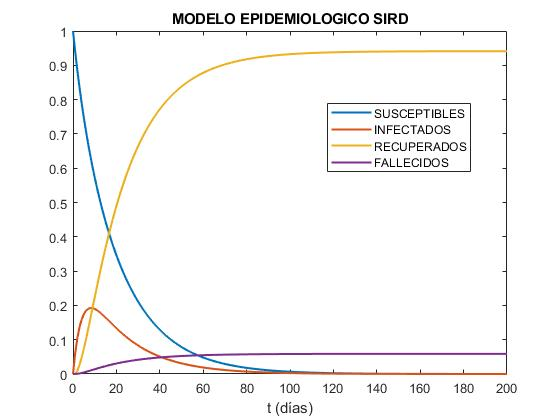
\includegraphics[width=0.8\textwidth]{Pictures/DIAG_EPIDEM.jpg}
 \end{figure}

\bigskip

Si se desea saber la evolución de la cantidad de individuos en cada estado después de 6 meses, se debe calcular $A^{180}$ !! 

Si $A$ fuera diagonal esto llevaría un  bajo costo computacional ya que quedarían elevados al exponente $180$  los elementos de la diagonal.



\bigskip

El prograna en lenguaje de programación GNU Octave que sigue diagonaliza la matriz $A$ del modelo. 
%Se sugiere al lector ejecutar  el programa  y comparar los tiempos de ejecución  para calcular $XF$ con la matriz $A$ y $XFD$ con la diagonalización.


\bigskip

% MODELO SIRD
% El 94% de la población sigue siendo susceptible. 6% adquiere la
% enfermedad
% El 1% morirá por la enfermedad, el 16% se recuperará y tendrá inmunidad. 
% El 3% se recuperará y no tendrá inmunidad, volverá a ser
% susceptible. El 80% seguirá infectado
% Los recuperados y los fallecidos permanecen en ese estado


\begin{lstlisting}[frame=single]
% MODELO SIRD 
%(SUSCEPTIBLES, INFECTADOS, RECUPERADOS, FALLECIDOS)
clear all
close all
A=[.94 .03 0 0 ; 0.06 .8 0 0 ; 0 0.16 1 0 ; 0 0.01 0 1];
X=[1 0 0 0 ]';
t=0:200;
for k= 1:200
    X(:,k+1)=A*X(:,k);
end
for k=1:4
%plot(t,X(k,:),'linewidth',1.5)
hold on
axis tight
end
XF=A^180
[U,D]=eig(A);
XFD=U*D^180*inv(U)
\end{lstlisting}

%[ht!]
\bigskip


\begin{remark}
Este ejemplo estuvo inspirado en la pandemia del COVID-19 del año 2020 y en estudios realizados en el tema, como el del trabajo \cite{covid}.  Los modelos matemáticos de epidemia que se utilizaron para su análisis  y para hacer predicciones  son modelos  de última generación,  representados mediante un sistema de ecuaciones diferenciales  con muchas variables y  poblaciones y que, entre otros  parámetros,  contemplan los que miden el comportamiento social. 
\end{remark}



En  la Sección \ref{cbaseTL} vimos, en el  Ejemplo \ref{ejemplo217}, que dada una aplicación lineal $T$ cuya matriz en la base canónica es 

$$T=\left(\begin{array}{cc}  6 & -2  \\ 6 &  -1
\end{array}
 \right)$$

\bigskip

\noindent
es posible hallar  una base tal que la matriz sea diagonal. 


$$T^\prime=\left(\begin{array}{cc}  2 & 0  \\ 0 &  3
\end{array}
\right)$$

\bigskip


La matriz $T^\prime$ en esa nueva base es mucho más sencilla que la matriz $T$ y se tiene que $T^\prime=C^{-1}TC$  donde $C$ es la matriz de cambio de base.
Nos surge  la pregunta si esto siempre es posible.


\bigskip


Un ejemplo sencillo que nos permite responder que no siempre es posible es la matriz 

$$T=\left(\begin{array}{cc}  1 & 1  \\ 0 &  1
\end{array}
 \right)$$

\bigskip


Supongamos existe una matriz $C$ de cambio de base  tal que 

\bigskip

$$C^{-1}TC=T^\prime=\left(\begin{array}{cc}  \alpha & 0  \\ 0 &  \beta
\end{array}
 \right)$$
 
\bigskip
\noindent
o en forma equivalente,

$$T=C\left(\begin{array}{cc}  \alpha & 0  \\ 0 &  \beta
\end{array}
 \right)C^{-1}$$ 
%ver H pag 284


\bigskip

$$\left(\begin{array}{cc}  1 & 1  \\ 0 &  1
\end{array}
 \right)= \left(\begin{array}{cc}  a & b  \\ c &  d
\end{array}
 \right) \left(\begin{array}{cc}  \alpha & 0  \\0 &  \beta
\end{array}
 \right) \left(\begin{array}{cc}  d & -b  \\ -c &  a
\end{array}
 \right) \frac{1} {Det(C)}$$

\bigskip

$$\left(\begin{array}{cc}  1 & 1  \\ 0 &  1
\end{array}
 \right)= \left(\begin{array}{cc}  a\alpha & b\beta  \\ c\alpha &  d\beta
\end{array}
 \right)  \left(\begin{array}{cc}  d & -b  \\ -c &  a
\end{array}
 \right) \frac{1} {Det(C)}$$
 
\bigskip 


$$\left(\begin{array}{cc}  1 & 1  \\ 0 &  1
\end{array}
 \right)= \left(\begin{array}{cc}  a\alpha d - b\beta c & -a\alpha b + b  \beta a \\ c \alpha d - c d \beta &  -c \alpha b +  d \beta a
\end{array}
 \right)   \frac{1} {Det(C)}$$

\bigskip

Igualando los elementos de ambas matrices, se tiene un sistema de ecuaciones:

\bigskip
\begin{eqnarray}
Det(C)&=& a\alpha d - b\beta c \\
Det(C)&=& ba( -\alpha  +   \beta )  \\
0&=&cd( -\alpha  +   \beta )  \\
Det(C)&=& -c \alpha b + d \beta a
\end{eqnarray}
 


\bigskip

\bigskip

De la igualdad $(3$.$3)$  se tiene que $c=0$ o $d=0$ o $\alpha = \beta$. Si $c=0$, de $(3$.$1)$ y ($3$.$4$), queda $Det(C)= a\alpha d= d \beta a$, de donde $\alpha = \beta$ y en $(3$.$3)$ se tiene $1=0$.
Si $d=0$, de $(3$.$1)$ y $3$.$4$,  $Det(C)= - b \beta c = -c\alpha b $, de donde también resulta $\alpha = \beta$ y en $(3.3)$ se tiene $1=0$. Lo mismo si $\alpha = \beta$. 

Se llega a una contradicción. Concluimos que no siempre es posible diagonalizar una matriz.

\bigskip

\begin{remark}
 \begin{itemize}
     \item 
No todas las matrices son diagonalizables.

\item 
Si es digonalizable,  $A$ es semejante a una matriz diagonal y tendremos ventaja al calcular su potencia. En otros casos  será semejante a una matriz casi diagonal.
  \item 
  Siempre es posible encontrar una forma \textit{ más sencilla} de una matriz dada  mediante un cambio de base. Se denomina \textit{matriz de Jordan de la matriz dada} y el nombre se debe al matemático Camille Jordan (1838-1922).
 \end{itemize}   
\end{remark}


\bigskip
Si se desea  calcular 

\bigskip

$$T^6=\left(\begin{array}{cc}  6 & -2  \\ 6 &  -1
\end{array}
 \right)^6$$

\bigskip
\noindent
como  $T=CT^\prime C^{-1}$,  $T^2=CT^\prime C^{-1} CT^\prime C^{-1}=CT^\prime I T^\prime C^{-1}=C(T^\prime)^2 C^{-1}$, y en general, 
$$T^n=C(T^\prime)^n C^{-1}, \quad n \in \mathbb{Z}$$
\noindent
de donde se tiene que 

\bigskip

$$T^6=\left(\begin{array}{cc}  1 & 2  \\ 2 &  3
\end{array}
 \right) \left(\begin{array}{cc}  2^6 & 0  \\ 0 &  3^6
\end{array}
 \right) \left(\begin{array}{cc}  -3 & 2  \\ 2 &  -1
\end{array}
 \right) $$

\bigskip

\section{Subespacios invariantes. Valores y vectores propios.}\index{Subespacios invariantes}
\label{Subespacios invariantes}


Dado un espacio vectorial $V$ y una aplicación lineal  $T: V \rightarrow V$, es decir $T \in L(V)$, un subespacio vectorial $W$ de $V$ se dice  \textit{invariante}   respecto a $T$ si $T(W)\subset W$, es decir si la imagen $T(\vec{x})$ de todo vector  $\vec{x}\in W$ es un elemento de $W$.

\bigskip

 %(es inyectiva si y sólo si  $N(T)=
\begin{example}

Sea $T\in L(\mathbb{R}^2)$ una aplicación lineal en $\mathbb{R}^2$ cuya matriz respecto de la base canónica $\left\{\vec{e_1} , \vec{e_2}\right\}$ de $\mathbb{R}^2$ está dada por 


$$T=\left(\begin{array}{cc}  2 & 0  \\ 0 &  1
\end{array}
\right)$$

\bigskip

Entonces $W_1=\left\{x_1\vec{e_1} ,~ x_1\in \mathbb{R}\right\}$ y $W_2=\left\{x_2\vec{e_2} ,~ x_2\in \mathbb{R}\right\}$ son invariantes respecto de $T$. 


\bigskip

En efecto, de la definición de matriz de una transformación lineal se tiene que $T(\vec{e_1})=2 \vec{e_1} + 0 \vec{e_2}$ y $T(\vec{e_2})=0 \vec{e_1} + 1 \vec{e_2}$.

\bigskip
Luego, 

$$T(x_1\vec{e_1})=x_1T(\vec{e_1})=x_1(2\vec{e_1})=(2x_1)\vec{e_1}\in W_1$$

y

$$T(x_2\vec{e_2})=x_2T(\vec{e_2})=x_2\vec{e_2}\in W_2$$

\end{example}
\bigskip

 %(es inyectiva si y sólo si  $N(T)=
\begin{example}

Sea $R_\alpha$ una rotación de ángulo $\alpha\neq 0$ en $\mathbb{R}^3$ con respecto al eje $z$. Geométricamente se observa que el plano $xy$ y el eje $z$ son invariantes con respecto a esta aplicación. Para comprobar algebraicamente que el plano $xy$ es invariante se observa, en primer lugar,  que la matriz de $R_\alpha$ con respecto a la base canónica de $\mathbb{R}^3$ es 


$$R=\left(\begin{array}{ccc} cos\alpha & -sen\alpha &  0 \\ sen\alpha & cos\alpha & 0
\\ 0 & 0 & 1
\end{array}
 \right).$$

\vskip0.25cm
Si $\vec{x}=x_1\vec{e_1}+ x_2\vec{e_2}$ es un elemento del plano $xy$, se tiene que su rotación da el vector



$$\left(\begin{array}{ccc} cos\alpha & -sen\alpha &  0 \\ sen\alpha & cos\alpha & 0
\\ 0 & 0 & 1
\end{array}
 \right)  \left(\begin{array}{c} x_1 \\ x_2
\\ 0 
\end{array}
 \right) =  \left(\begin{array}{c} x_1cos\alpha- x_2sen\alpha  \\ x_1sen\alpha+ x_2cos\alpha 
\\ 0 
\end{array}
 \right)   $$

 \bigskip
\noindent 
y, por lo tanto, $R_\alpha(\vec{x})= (x_1cos\alpha- x_2sen\alpha)\vec{e_1}+  (x_1sen\alpha+ x_2cos\alpha) \vec{e_2}     $  y  es nuevamente un elemento del plano $xy$.

\end{example}
\begin{figure}[ht]
    \centering
    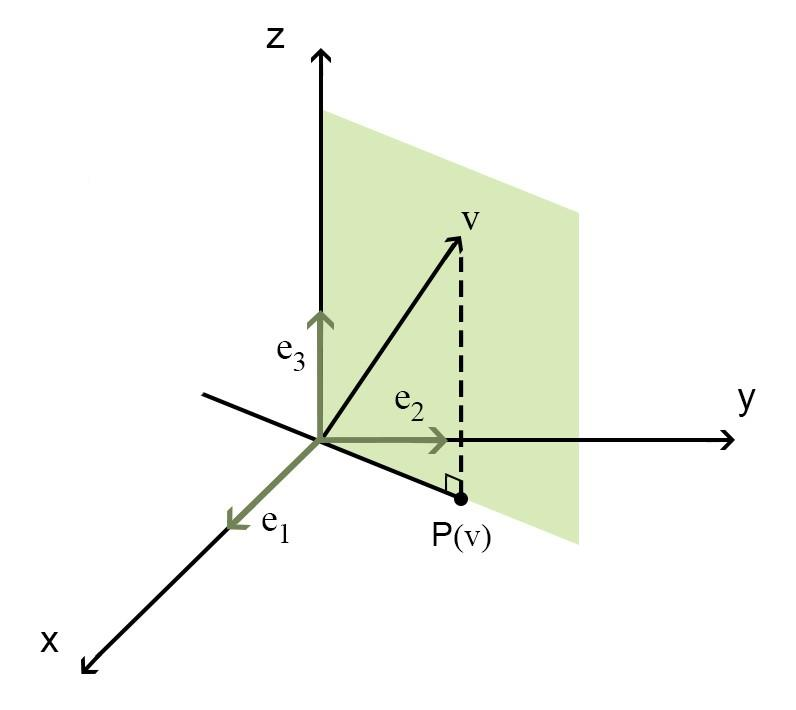
\includegraphics[width=0.70\textwidth]{Pictures/fig.35.jpg}
    \caption{Todo plano que contiene al eje $z$ es invariante por $P$.
    }
    \label{pag286}
\end{figure}

\bigskip

\begin{example}

En la Figura \ref{pag286} se muestra   la proyección ortogonal $P$ de $\mathbb{R}^3$  sobre el plano $xy$. (Ver Ejemplo \ref{proyxy}). La matriz de $P$ es 
$$P=\left(\begin{array}{ccc} 1 & 0 &  0 \\ 0 & 1 & 0
\\ 0 & 0 & 0
\end{array}
 \right)$$
con respecto a la base canónica. Se puede ver que todo plano $\pi$  que contiene al eje $z$ es invariante:

\noindent
el plano  $\pi$ tiene ecuación $x_1 x +  x_2 y + x_3 z=0$, donde $x_3=0$ ya que $(0,0,1) \in \pi$. Los vectores de ese plano  son de la forma
$\vec{x}=x_1\vec{e_1} + \lambda x_1\vec{e_2} + x_3\vec{e_3}, ~\lambda \in \mathbb{R}$,
y se  tiene que su imagen, $P(\vec{x})$,  es de nuevo un elemento del plano $\pi$:
$$P=\left(\begin{array}{ccc} 1 & 0 &  0 \\ 0 & 1 & 0
\\ 0 & 0 & 0
\end{array}
 \right)      \left(\begin{array}{c} x_1 \\ \lambda x_1
\\ x_3
\end{array}
 \right) =   \left(\begin{array}{c} x_1 \\ \lambda x_1
\\ 0
\end{array}
 \right)            $$



\bigskip
% agregar figura de la pág. 286 VH




Otros subespacios invariantes de esta proyección ortogonal son el plano $xy$, el eje $z$ y cualquier recta del plano $xy$ que pase por el origen de coordenadas.
\end{example}

\bigskip

\begin{remark}
Para cualquier transformación lineal  $T\in L(V)$ ( o endomorfismo), el subespacio $S=\left\{\vec{0}\right\}$, formado sólo por el elemento nulo, es invariante ya que $T(\vec{0})=\vec{0}$ y el propio espacio vectorial $V$ es también invariante ya que $T(\vec{x})$ para todo vector  $\vec{x}\in V$ es un elemento de $V$.
%\hfill$\blacktriangle$
\end{remark}

\bigskip

\begin{theorem}
\label{intysumainv}
\noindent
La intersección y la suma de subespacios invariantes respecto de una aplicación lineal $T\in L(V)$ son subespacios invariantes respecto de $T$.

%\begin{proof}
Se deja la demostración al lector.
%\end{proof}

\end{theorem} 

\bigskip

\bigskip

\bigskip


\begin{definition}\index{Autovector (o vector propio)}\index{Autovalor (o valor propio)}
%\label{eigen}

\bigskip

Un vector $\vec{v}\neq \vec{0}$ de un espacio vectorial $V$ sobre $K$ se llama \textit{autovector} o \textit{vector propio}  de una aplicación lineal $T\in L(V)$ si existe un escalar $\lambda \in K$ tal que $T(\vec{v})=\lambda \vec{v}$. Este número $\lambda $ se denomina \textit{autovalor }o \textit{valor propio} de la aplicación $T$ correspondiente al vector $\vec{v}$.

\end{definition}

\bigskip

\begin{remark}
Si $\vec{v}$  es un vector propio de $T$ con autovalor  $\lambda$, todo elemento no nulo del subespacio unidimensional generado por $\vec{v}$ es un autovector de $T$ con el mismo autovalor $\lambda $. Esto es porque $T(c \vec{v})=c T(\vec{v})= c \lambda \vec{v}=\lambda (c\vec{v}) $.
%\hfill$\blacktriangle$
\end{remark}
\bigskip



\begin{figure}
    \centering
    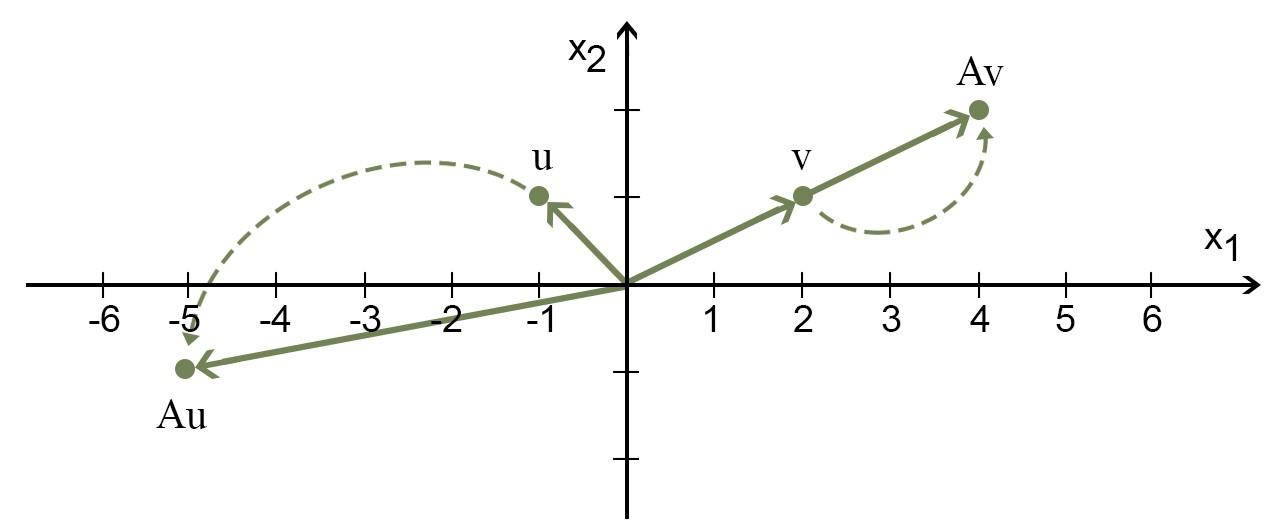
\includegraphics[width=0.90\textwidth]{Pictures/FIGAuAv.jpg}
    \caption{El vector $\vec{v}$ es autovector de $A$, mientras que el vector $\vec{u}$ no es autovector,   $A\vec{u}$  no es múltiplo de $\vec{u}$.}
    \label{FIGAuAv}
\end{figure}

\bigskip

\begin{theorem}
\label{PROPOSICION3}
Una aplicación lineal  $T\in L(V)$ es diagonalizable sí y sólo sí existe una base de $V$ formada por vectores propios.

\begin{proof}

Supongamos que una aplicación lineal $T$ en un espacio $V$ de dimensión $n$ tiene $n$ vectores propios linealmente independientes, $\vec{e}_1,\vec{e}_2, \cdots ,\vec{e}_n$ con valores propios $\lambda_1,\lambda_2, \cdots ,\lambda_n$ respectivamente, tomando $\left\{\vec{e}_1,\vec{e}_2, \cdots,\vec{e}_n\right\}$ como una base de $V$ se tiene que 

$$T(\vec{e}_1)=\lambda_1\vec{e}_1, T(\vec{e}_2)=\lambda_2\vec{e}_2, \cdots,T(\vec{e}_n)=\lambda_n\vec{e}_n$$

\bigskip

\noindent
y, por lo tanto, la matriz de $T$ con respecto a esta base es la matriz diagonal

\bigskip


$$T=\left(\begin{array}{ccccc} \lambda_1 & 0 &  0 & 0 &  0\\ 0 &  \lambda_2 & 0  & 0 & 0
\\ 0 & 0  &\ddots   &  0 &   0  \\   0 & 0 &  0 &\ddots   &  0   \\ 0 & 0 & 0 & 0 & \lambda_n
\end{array}
 \right)$$



\bigskip


Recíprocamente, toda aplicación lineal que tiene una matriz diagonal en una cierta base, tiene a los elementos de esta base como vectores propios. 


\bigskip


\end{proof}

\end{theorem}

\bigskip

\begin{remark}
Una aplicación lineal  $T\in L(V)$ es \textit{diagonalizable} sí y solo sí existe una base de $V$ en la cual la matriz de $T$ es diagonal.
%\hfill$\blacktriangle$
\end{remark}


\begin{definition}\label{Diag}\index{Matriz diagonalizable}

Una matriz $T\in K^{n \times n}$ se dice diagonalizable en $K$ si la aplicación lineal  $T: K^n \rightarrow  K^n$ que la matriz que la representa es diagonalizable.

\end{definition}

\bigskip
\noindent
De esta definición se deduce que una matriz es diagonalizable en $K$ si existe una matriz $C\in K^{n \times n}$ con determinante no nulo, tal que $T^\prime=C^{-1}TC$ es una matriz diagonal.

\bigskip





\noindent
En el ejemplo del inicio de la sección, para 

$$T=\left(\begin{array}{cc}  6 & -2  \\ 6 &  -1
\end{array}
 \right)$$
 \noindent
se tiene que 
 
 
$$\left(\begin{array}{cc}  6 & -2  \\ 6 &  -1
\end{array}
 \right) \left(\begin{array}{c}  1   \\ 2 
\end{array}
 \right) = \left(\begin{array}{c}  2  \\ 4 
\end{array}
 \right)  = 2 \left(\begin{array}{c}  1  \\ 2 
\end{array}
 \right)  $$
 
\bigskip

$$\left(\begin{array}{cc}  6 & -2  \\ 6 &  -1
\end{array}
 \right) \left(\begin{array}{c}  2   \\  3
\end{array}
 \right) = \left(\begin{array}{c}  6  \\ 9 
\end{array}
 \right)  = 3 \left(\begin{array}{c}  2  \\ 3 
\end{array}
 \right)  $$

\bigskip

Se tiene que $T(\vec{v}_1)=  2 \vec{v}_1$ y  $T(\vec{v}_2)=  3 \vec{v}_2$, siendo    $\vec{v}_1=(1, 2)$ y $\vec{v}_2=(2, 3)$, con lo que $\vec{v}_1 $ y $ \vec{v}_2$ son vectores propios de $T$ con sus correspondientes valores propios $2$ y $3$ respectivamente.
Como $\vec{v}_1$ y $\vec{v}_2$  forman una base de $\mathbb{R}^2$ (son linealmente independientes y son $2$), la matriz $T$ es diagonalizable en $\mathbb{R}$ y su matriz diagonal asociada es 

$$\left(\begin{array}{cc}  2 & 0  \\ 0 &  3
\end{array}
 \right)$$
 
\bigskip


\noindent
\textbf{Cálculo de  autovalores y autovectores de una transformación lineal.}

\bigskip

Supongamos que $\vec{v}$ es un vector propio de una aplicación lineal $T$ en un espacio vectorial $V$ y que $\lambda$ es su autovalor, es decir $T(\vec{v})=\lambda \vec{v}$. Sea $\left\{\vec{e}_1,\vec{e}_2, \cdots,\vec{e}_n\right\}$ una base de $V$ y  sean   $v_{j}$, $ j=1,\cdots n $ las coordenadas de  $\vec{v}$ en esa base, es decir,  $\vec{v}=\sum_{j=1}^{n}v_{j}\vec{e}_j$. Si $(a_{ij})$ es la matriz 
de $T$ con respecto a la base tenemos que 


$$\sum_{j=1}^{n} \lambda v_{j}\vec{e}_j = \lambda \sum_{j=1}^{n}  v_{j}\vec{e}_j = \lambda \vec{v}=T(\vec{v})=T(\sum_{j=1}^{n}  v_{j}\vec{e}_j) $$

%\newpage

\bigskip


$$ =\sum_{j=1}^{n}  v_{j} T(\vec{e}_j )= \sum_{j=1}^{n}  v_{j}  (\sum_{i=1}^{n}  a_{ij}\vec{e}_i)=  \sum_{i=1}^{n}   (\sum_{j=1}^{n}  a_{ij} v_{j})\vec{e}_i $$

\bigskip

Como $\left\{\vec{e}_1,\vec{e}_2, \cdots,\vec{e}_n\right\}$ es una base de $V$, del primer y del último término de la igualdad anterior se tiene que: 

\bigskip

\begin{equation} \label{matriz A0}
\left\{ \begin{array} {ccl} 
                    \lambda v_1&=&a_{11}v_1+a_{12}v_2+\cdots +a_{1n}v_n    \\
                    \lambda v_2&=&a_{21}v_1+a_{22}v_2+\cdots +a_{2n}v_n  \\
										\cdots  \\
                    \lambda v_n&=&a_{n1}v_1+a_{n2}v_2+\cdots +a_{nn}v_n  
                   \end{array}
           \right.
\end{equation}

\bigskip

\noindent
o en forma equivalente,

\bigskip

\begin{equation} \label{matriz A}
\left\{ \begin{array} {ccl} 
                    (a_{11}-\lambda)v_1+a_{12}v_2+\cdots +a_{1n}v_n  =& 0  \\
                    a_{21}v_1+(a_{22}-\lambda)v_2+\cdots +a_{2n}v_n =& 0 \\
										\cdots  \\
                    a_{n1}v_1+a_{n2}v_2+\cdots +(a_{nn}-\lambda)v_n  =& 0
                   \end{array}
           \right.
\end{equation}

\bigskip


Como es un sistema homogéneo, para que exista una solución no nula debe ocurrir que 

\bigskip

\begin{equation} \label{polca}
Det(A-\lambda I)=\left(\begin{array}{cccccc}a_{11}-\lambda & a_{12} & a_{13} &\cdots  &\cdots & a_{1n}\\ a_{21} & a_{22}-\lambda    &\cdots  &\cdots  &\cdots &a_{2n}
\\\cdots & \cdots   &\ddots   &  \cdots  &   \cdots   \\ \cdots & \cdots  & \cdots  &  \ddots  &\cdots   & \cdots  
\\ \cdots & \cdots  & \cdots  &  \cdots  &\ddots   & \cdots 
\\ a_{n1} & a_{n2}  &  &\cdots  &  a_{nn-1} & a_{nn}-\lambda
\end{array}
 \right) =  0
\end{equation}

\bigskip

\noindent
donde $I$ denota la matriz identidad. Esto es una ecuación de grado $n$ en $\lambda$ y sus soluciones en $K$ ($\mathbb{R}$ o $\mathbb{C}$) son los autovalores de $T$. 
Si $V$ es un espacio vectorial complejo, por el teorema fundamental del álgebra la ecuación anterior tiene $n$ soluciones complejas contando cada una con su multiplicidad. Si $V$ es un espacio vectorial real, no podemos asegurar que la ecuación anterior tenga $n$ soluciones reales.


\bigskip
%En base a lo anterior, los 
{\textbf{Pasos para resolver $A\vec{v}=\lambda \vec{v}$}}

\bigskip

\begin{enumerate}
\item
Se calcula $ Det(A-\lambda I)$ (se anota en forma equivalente como $\left   | A -  \lambda I   \right  |$)      , restando $ \lambda $ de los elementos de la diagonal de la matriz $A$. Es un polinomio de grado $n$, con coeficiente $ (-\lambda)^n $. 

\bigskip

\item
Se hallan las raíces de este polinomio. Las $n$ raíces son los autovalores de la matriz $A$.

\bigskip

\item
Para cada autovalor $ \lambda $, se resuelve el sistema lineal  $(A-\lambda I) \vec{v}=   \vec{0} $. Como el determinante es cero, tendrá soluciones no nulas. Esos son los autovectores.


\end{enumerate}


\bigskip

\bigskip

\begin{example}
\label{ejemploaut}
\noindent
Se desea determinar los valores y vectores propios de la aplicación lineal de $T: V \rightarrow V$, $V=\mathbb{R}^2$, que tiene como matriz, 

\bigskip

$$T=\left(\begin{array}{cc}  1 & 2  \\ 5 &  4
\end{array}
 \right)$$

\begin{enumerate}
\item
\[
0= 
\left   | T -  \lambda I   \right  |=\left | \begin{array}{cc}
1- \lambda  & 2  \\
5 &  4- \lambda 
\end{array}
\right|=(1- \lambda)(4- \lambda)-10= \lambda^2 - 5 \lambda -6
\]


\bigskip

\item
Las raíces son $\lambda_1= 6$ y $\lambda_2=-1$

\bigskip


\item

Para $\lambda_1= 6$  se resuelve el sistema 

$$(T-6I) \left(\begin{array}{c}  x_1  \\ x_2 
\end{array}
 \right)=  \left(\begin{array}{c}  0  \\ 0 
\end{array}
 \right) $$

 Los vectores propios correspondientes a $\lambda_1= 6$  son de la forma $ \alpha  \left(\begin{array}{c}  2  \\ 5 
\end{array}
 \right)$.

\bigskip

 
Para $\lambda_2= -1$  se resuelve el sistema 

$$(T-(-1)I) \left(\begin{array}{c}  x_1  \\ x_2 
\end{array}
 \right)=  \left(\begin{array}{c}  0  \\ 0 
\end{array}
 \right) $$

 Los vectores propios correspondientes a $\lambda_2= 6$  son de la forma $ \beta  \left(\begin{array}{c}  1  \\ -1 
\end{array}
 \right)$.
 \end{enumerate}
 
\bigskip


 Como $  \left(\begin{array}{c}  2  \\ 5 
\end{array}
 \right)$  y $  \left(\begin{array}{c}  1  \\ -1 
\end{array}
 \right)$  forman una base de $\mathbb{R}^2$, por la Proposición \ref{PROPOSICION3},  $T$ es diagonalizable, 
 
 \bigskip

 \bigskip
 
 \noindent
 con matriz diagonal 

 $$\left(\begin{array}{cc}  6 & 0  \\ 0 &  -1
\end{array}
 \right)$$
 
 \bigskip

 
\noindent
 y la matriz de  cambio de base (de la base de autovectores a la base canónica) está dada por la matriz

 $$C=\left(\begin{array}{cc}  2 & 1  \\ 5 &  -1
\end{array}
 \right)$$
\end{example}


\bigskip
\index{Strang, William Gilbert}
\begin{parchment}[William Gilbert Strang  (1934)] {Es un matemático estadounidense, actualmente Professor Mathworks de Matemáticas del Department of Mathematics del Massachusetts Institute of Technology (MIT). Ha contribuido a la teoría de elementos finitos, al cálculo de variaciones, al análisis wavelet y al  álgebra lineal. Ha contribuido enormemente a la educación en matemáticas, en forma de libros técnicos y cursos online. En MIT enseña Álgebra Lineal, Ciencia Computacional e Ingeniería, Aprendiendo de los Datos. Sus clases están disponibles en la plataforma MIT OpenCourseWare (en inglés).
Gilbert Strang nació en Chicago, Illinois. Cursó estudios en el propio MIT y en el Balliol College, en la Universidad de Oxford. Se doctoró en la Universidad de California, Los Ángeles (UCLA) y desde ese momento ha llevado a cabo su actividad docente en el MIT. Entre las publicaciones más notables del Professor Strang se destaca An Analysis of the Finite Element Method, conjuntamente con George Fix, así como seis manuales:
Introduction to Linear Algebra (1993, 1998, 2003),
Linear Algebra and Its Applications (1976, 1980, 1988, 2005),
Introduction to Applied Mathematics (1986),
Calculus (1991),
Wavelets and Filter Banks, con Truong Nguyen (1996),
Linear Algebra, Geodesy, and GPS, con Kai Borre (1997).

Gilbert Strang fue Presidente de la SIAM (Society for Industrial and Applied Mathematics) durante los años 1999-2000. También ha sido Chairman of the US National Committee on Mathematics durante los años 2003-2004. Es Honorary Fellow, en el Balliol College de Oxford. También es Chairman, en la National Science Foundation (NSF) del Advisory Panel del área de Matemáticas.

Fue pionero al abrir sus clases y permitir que fueran grabadas en vídeo mientras explicaba matemáticas a sus alumnos del MIT para su difusión abierta y gratuita en Internet. \cite{gstrang}}
\end{parchment}


%\newpage

\bigskip

%Completar del hernández pág 290


\subsection{Localización de autovalores}\index{Localización de autovalores}

\bigskip

\begin{corollary}
\label{Teodiscos}
Teorema de Gershgorin. \index{Gershgorin}

Los autovalores de una matriz $A$ están en la unión de los discos $D_1$, $D_2$, $\cdots$, $D_n$ (del plano complejo) donde $D_i$ es el disco centrado en el elemento de la diagonal $a_{ii}$: 

$$|\lambda-a_{ii}|  \leq  r_i  $$

Su radio $r_i=\sum_{j \neq i} |a_{ij}|$ es igual a la suma de los valores absolutos de los elementos del resto de la fila.


\begin{proof}
Supongamos $v_i$ es la mayor componente en valor absoluto del autovector  $\vec{v}$,  $ A\vec{v}=\lambda \vec{v}$. Entonces,

\bigskip

$(\lambda-a_{ii})v_i= \sum_{j \neq i} a_{ij} v_j$, de donde, 

\bigskip

$|\lambda-a_{ii}|  \leq  \sum_{j \neq i} |a_{ij}| \frac{   |v_j|}{ |v_i| } \leq  \sum_{j \neq i} |a_{ij}|=r_i  $

\end{proof}
\end{corollary}

\bigskip


\begin{example}
Dada la matriz,

\bigskip

$$A=\left(\begin{array}{cccc} 3 & 0 &  -1 & 1/2 \\ 0 & 5   & 1/2 & 1
\\  -1/2  &  0 &  -3 &   5/4

\\   0 & 1/2 &  1/2 & 4 
\end{array}
 \right)$$

 \bigskip

 
Se muestra en la Figura \ref{DISCOS} la localización de sus autovalores de acuerdo al Teorema \ref{Teodiscos}. Los discos están centrados en los elementos de la diagonal de la matriz $A$ y tienen radios $r_1=3/2$, $r_2=3/2$, $r_3=7/4$ y $r_4=1$. Están en el intervalo $[-19/4,7]$, en el caso que sean números reales.

 \bigskip
 
\begin{figure}
    \centering
    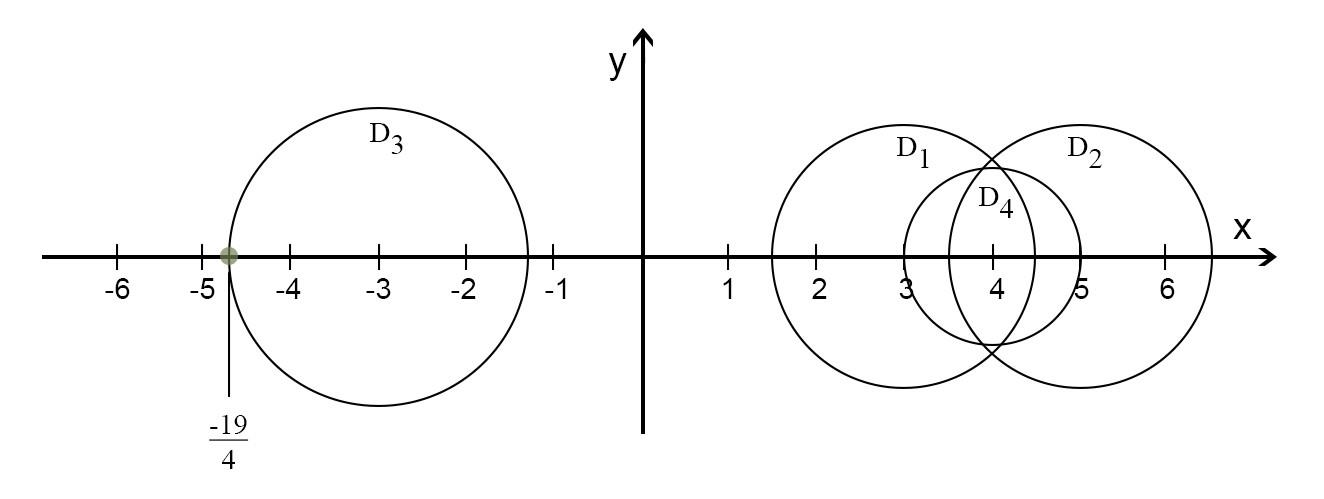
\includegraphics[width=0.90\textwidth]{Pictures/DISCOS.jpg}
    \caption{Los autovalores de $A$ se encuentran en la unión de los cuatro discos, $D_1, D_2, D_3$ y $D_4$.}
    \label{DISCOS}
\end{figure}


\end{example}
\bigskip

Para la matriz del Ejemplo \ref{ejemploaut} se  tienen los discos  $D_1=|\lambda-1|  \leq 2$ y $D_2=|\lambda-4|  \leq 5$.  Sin calcular los autovalores, se sabe que si son números reales, estarán  en el intervalo $[-1,9]$.


\section{Polinomio característico}
\label{polcar}

Al polinomio $Det(T-\lambda I) \in P_K^{(n)}\left[\lambda\right]$  (Ec. (\ref{polca})) se lo denomina \textit{polinomio característico} de la aplicación $T$  (o de la matriz $A \in K^{n \times n}$). Lo anotaremos  $\mathbf{P}_T( \lambda) $.

\bigskip

\begin{theorem}
\label{proppolauto}

Sea $T\in K^{n \times n}$ y sea $\lambda \in K$. Entonces $\lambda$ es autovalor de $T$ sí y sólo sí $\lambda$ es raíz del polinomio característico de $T$.


\end{theorem}

\bigskip

\begin{example}
La matriz 
$$\left(\begin{array}{cc}  0 & 1  \\ -1 &  0
\end{array}
 \right)$$

 \bigskip
\noindent 
es diagonalizable en $\mathbb{C}^{n \times n}$, pero no es diagonalizable en $\mathbb{Q}^{n \times n}$ ni en $\mathbb{R}^{n \times n}$. Sus autovalores son las raíces del polinomio


$$Det\left(\begin{array}{cc}  0-\lambda  & 1  \\ -1 &  0-\lambda
\end{array}
 \right)= \lambda^2+1=0 $$

\bigskip

Se tiene, entonces, que los autovalores son $\lambda_{1-2}= \mp i$
%y no dependen de la base elegida.
\end{example}






\bigskip


\begin{theorem}
\label{polcarbase}
El polinomio característico no depende de la base elegida en $V$ para representar la aplicación lineal  $T$.


\begin{proof}


\noindent
Sea $\mathbf{P}_{T,B}(\lambda)=Det(T-\lambda I)$ el polinomio característico  de la aplicación $T$ en la base $B=\left\{\vec{e}_1,\vec{e}_2, \cdots,\vec{e}_n\right\}$  de $V$ y sea  $\mathbf{P}_{T,B^{\prime}}(\lambda)=Det(T^{\prime}-\lambda I)$ el polinomio característico de $T$ en la base $B^{\prime} =\left\{\vec{e ^{\prime}}_1,\vec{ e ^{\prime}}_2,\cdots, \vec{e^{\prime}}_m\right\}$; si $C$ es la matriz del cambio de base, se  sabe que    $T=CT^\prime C^{-1}$, 
y se tiene 

\bigskip

$$\mathbf{P}_{T,B}(\lambda)=\mathbf{P}_{T,B^{\prime}}(\lambda)$$  

Se deja al lector  completar esta demostración.

\end{proof}
\end{theorem}

\bigskip

\bigskip

\begin{example}
La matriz de la proyección sobre el eje $x$, $ P_x$, (Ver Ejemplo \ref{proyejex}) en la base canónica $B=\{\vec{e}_1, \vec{e}_2 \}  $ es 

$$\left(\begin{array}{cc}  1 & 0  \\ 0 &  0
\end{array}
 \right)$$

 \bigskip
 
 Los autovalores son $\lambda_1=1$ y $\lambda_2=0$, ya que para los vectores $\vec{v}_1$ que están sobre el eje $x$ se verifica $P_x(\vec{v}_1)=1\vec{v}_1$, mientras que para los los vectores $\vec{v}_2$ que están sobre el eje $y$ se verifica $P_x(\vec{v}_2)=\Vec{0}$.
 
\bigskip
Si cambio de base, por ejemplo a la base $B^{\prime}= \{\vec{e}_1^{\prime}, \vec{e}_2^{\prime} \} $ (rotando  en $ \phi= \pi/4$ los vectores de la base canónica $B$),  donde los vectores de $B^{\prime}$ son las columnas de la matriz $A$ del Ejemplo \ref{ejrotR2}, se tendrá que 

$$ P_x( \vec{e}_1^{\prime})=(\sqrt 2/2,0)= 1/2 \vec{e}_1^{\prime} -1/2 \vec{e}_2^{\prime} $$
y 

$$ P_x( \vec{e}_2^{\prime})=(-\sqrt 2 /2,0)= -1/2 \vec{e}_1^{\prime} +1/2 \vec{e}_2^{\prime} $$

\noindent
entonces la matriz en esta nueva base es

$$\left(\begin{array}{cc}  1/2 & -1/2  \\ -1/2 &  1/2
\end{array}
 \right)$$

 \bigskip

 Ahora el polinomio característico es $\mathbf{P}_{P_x,B^{\prime}}(\lambda)(1/2-\lambda)^2 -1/4$, con las mismas raíces, $\lambda_1=1$ y $\lambda_2=0$, y los mismos autovectores que se obtuvieron con la base $B$, ya que

 \bigskip
 
 $\vec{v}^{\prime}_1= (1,-1)_{B^{\prime}}= 1(\sqrt 2 /2,\sqrt 2 /2)-1(-\sqrt 2 /2,\sqrt 2 /2)=(1,0)$ y
 
 \bigskip
 
 $\vec{v}^{\prime}_2= (1,1)_{B^{\prime}}=1(\sqrt 2 /2,\sqrt 2 /2)+1(-\sqrt 2 /2,\sqrt 2 /2)=(0,1)$.

 \bigskip
 
 Se verifica, entonces, como se vió en la  Observación 
 \textcolor{blue}{{\fontfamily{qcr}\selectfont{i}}} en  \ref{Obssemejanza} que las matrices de una misma transformación lineal en distintas bases son semejantes.  
Se tiene la relación, 

\bigskip

$$\left(\begin{array}{cc}  1 & 0  \\ 0 &  0
\end{array}
 \right)=  P _{B,B^{\prime}} \left(\begin{array}{cc}  1/2 & -1/2  \\ -1/2 &  1/2
\end{array}
 \right)P _{B^{\prime},B}$$
 
\bigskip
 
\noindent
 donde $P _{B,B^{\prime}}$ y $P _{B^{\prime},B}$ son las matrices del cambio de base de $B^{\prime}$ a $B$ y de $B$ a 
 $B^{\prime}$, respectivamente.
  \end{example}
  
 \bigskip
 
\begin{example}
\label{rotautov}


Se quieren determinar los valores y vectores propios de la aplicación lineal que corresponde a la rotación de ángulo $\alpha$ que tiene como matriz: (ver la matriz \ref{matrizrotR2}, Ejemplo  \ref{ejrotR2} )

\bigskip



$$R_\alpha=\left(\begin{array}{cc}  cos(\alpha) &-sen(\alpha)  \\ sen(\alpha) & cos(\alpha)
\end{array}
 \right)$$
\noindent
con respecto a la base canónica de $\mathbb{R}^2$.



\[
0= 
\left   | R_\alpha -   \lambda I \right  | = \left|\begin{array}{cc}
 cos(\alpha)-\lambda  & -sen(\alpha) \\
sen(\alpha) &  cos(\alpha)- \lambda 
\end{array}
\right| \]
\[=(cos(\alpha)- \lambda)^2+ sen^2(\alpha)= \lambda^2 - 2 cos(\alpha )\lambda +1
\]

\bigskip

Las raíces son $\lambda_1= cos(\alpha) + i sen(\alpha)$ y $\lambda_2= cos(\alpha) - i sen(\alpha)$, que son números complejos a no ser que $ \alpha = 2k \pi $ o $ \alpha = (2k+1) \pi $, con $k \in \mathbb{Z}$.

\bigskip

Si $ \alpha = 2k \pi $, se tiene la matriz identidad  y todo vector de $\mathbb{R}^2$ es autovector, y corresponden a $ \lambda=1$. 

\bigskip

Mientras que si $ \alpha = (2k+1) \pi $, la matriz es $-I$ y también resulta autovector cualquier vector de $\mathbb{R}^2$, y corresponden a $ \lambda=-1$. En este caso la transformación es una simetría respecto al origen de coordenadas.
\end{example}

\bigskip

\begin{example}
\noindent
La matriz correspondiente a una rotación de ángulo $\alpha$ en $\mathbb{R}^3$ con respecto al eje $z$, es,

$$R=\left(\begin{array}{ccc} cos(\alpha) & -sen(\alpha) &  0 \\ sen(\alpha) & cos(\alpha) & 0
\\ 0 & 0 & 1
\end{array}
 \right)$$

\bigskip

 Su polinomio característico es $  (\lambda^2 - 2 (cos(\alpha) )\lambda +1)(1-\lambda)$, cuyas raíces  son $\lambda_1= cos(\alpha) + i sen(\alpha)$, $\lambda_2= cos(\alpha) - i sen(\alpha)$ y $ \lambda_3= 1$.


\bigskip

Los vectores propios correspondientes a  $ \lambda_3= 1$ son las soluciones del sistema:
 
 \begin{eqnarray}
 \label{sisr3rot}
\left(\begin{array}{ccc} cos(\alpha) -1 & -sen(\alpha) &  0 \\ sen(\alpha) & cos(\alpha)-1 & 0
\\ 0 & 0 & 1
\end{array}
 \right)  \left(\begin{array}{c} x_1\\ x_2
\\ x_3
\end{array}
 \right) =  \left(\begin{array}{c} 0\\ 0
\\ 0
\end{array}
 \right) 
\end{eqnarray} 

 \bigskip
 
 Dado que 
\[
 \left|\begin{array}{cc}
 cos(\alpha)-1  & -sen(\alpha) \\
sen(\alpha) &  cos(\alpha)- 1 
\end{array}
\right|\]
\[=(cos(\alpha)- 1)^2+ sen^2(\alpha)= 2 - 2 cos(\alpha) =  4 sen^2 (\alpha /2 )
\]
El sistema (\ref{sisr3rot}) tiene únicamente la solución $x_1=x_2=0 $  si $ \alpha \neq 2k \pi $, con $k \in  \mathbb{Z}$. En este caso los autovectores correspondientes a $\lambda_3= 1$, son los vectores sobre el eje $z$, de la forma $(0,0,x_3)$.

\bigskip

Si $ \alpha = 2k \pi $, se trata de la identidad y todos los vectores de $ \mathbb{R}^3$ son autovectores.

\bigskip

Si $ \alpha = (2k+1) \pi $, $ $ $\lambda_1=\lambda_2= -1$, y los autovectores son las soluciones del sistema 

\bigskip

$$\left(\begin{array}{ccc} 0 & 0&  0 \\ 0 & 0 & 0
\\ 0 & 0 & 2
\end{array}
 \right)  \left(\begin{array}{c} x_1\\ x_2
\\ x_3
\end{array}
 \right) =  \left(\begin{array}{c} 0\\ 0
\\ 0
\end{array}
 \right)$$
 
\bigskip
\noindent
y son los vectores  $ (x_1, x_2,0)$ o sea del plano $xy$, y la transformación es una simetría respecto al eje $z$.

\end{example}

\bigskip



\section{Diagonalización.}
\label{diago}

La Proposición \ref{PROPOSICION3} nos da una condición necesaria y suficiente para saber cuándo una aplicación lineal es diagonalizable, a saber, que exista una base del espacio vectorial $V$ formada por vectores propios. En algunos casos puede resultar laborioso encontrar esta base. Una condición que es suficiente para poder asegurar la diagonalizaciónde una matriz está contenida en la proposición siguiente:



\bigskip


\begin{theorem}

\label{PROPOSICION4}



Los vectores propios de una aplicación $T$ correspon-\ dientes a valores propios distintos dos a dos, son linealmente independien-\ tes.

\begin{proof}
%ver hojita 27
Por inducción sobre la cantidad de vectores. 
\begin{itemize}
\item

Para $k=2$.
Supongamos que  se tienen $\Vec{v}_1$ correspondiente a $ \lambda_1 $ y $\Vec{v}_2$ correspondiente a $ \lambda_2 $, con $ \lambda_1  \neq \lambda_2 $.  

Si se tiene
\begin{eqnarray}
\label{auton2li}
 \alpha_1 \Vec{v}_1 + \alpha_2 \Vec{v}_2 &= &\Vec{0} \\
 T(\alpha_1 \Vec{v}_1 + \alpha_2 \Vec{v}_2 )&=&T( \Vec{0})=\Vec{0} \nonumber\\
\alpha_1 T(\Vec{v}_1) + \alpha_1 T(\Vec{v}_2 )&=&\Vec{0} \nonumber\\
\alpha_1 \lambda_1\Vec{v}_1 + \alpha_1 \lambda_2\Vec{v}_2 &=&\Vec{0} \nonumber
\end{eqnarray}

\bigskip

 De (\ref{auton2li}) se tiene que  $  \alpha_2 \Vec{v}_2 = - \alpha_1 \Vec{v}_1$. Si se reemplaza en la última ecuación, se tiene que
\begin{eqnarray}
 \alpha_1 \lambda_1\Vec{v}_1 - \alpha_1 \lambda_2 \Vec{v}_1 &=&\Vec{0} \nonumber\\
 \alpha_1 \Vec{v}_1( \lambda_1 - \lambda_2) &=&\Vec{0} 
 \end{eqnarray}


\bigskip 

 Como $\Vec{v}_1 \neq \Vec{0}$ y $ \lambda_1 - \lambda_2 \neq  0$, resulta  $ \alpha_1=0$, de donde  $ \alpha_2=0$, pues
 $\Vec{v}_2 \neq \Vec{0}$.

 \bigskip 
 
 Por lo tanto, $\Vec{v}_1$ y $\Vec{v}_2$ son linealmente independientes.


  \bigskip 
  
\item

Supongamos ahora el resultado es válido para $k-1$ autovalores distintos.

Si 

$\alpha_1 \Vec{v}_1 + \alpha_2 \Vec{v}_2  + \cdots + \alpha_{k-1} \Vec{v}_{k-1} + \alpha_{k} \Vec{v}_{k} = \Vec{0},$

\bigskip

como en el caso $k=2$, aplicamos $T$, despejamos de la igualdad anterior el término $\alpha_{k} \Vec{v}_{k}$. 

Entonces,

\bigskip 

$ \alpha_1 \lambda_1\Vec{v}_1 + \alpha_2 \lambda_2\Vec{v}_2 + \cdots  +\alpha_{k-1} \lambda_{k-1}\Vec{v}_{k-1}+  \alpha_{k} \lambda_{k}\Vec{v}_{k}=  \Vec{0} $

\bigskip

$ \alpha_1 \lambda_1\Vec{v}_1 + \alpha_2 \lambda_2\Vec{v}_2 + \cdots  +\alpha_{k-1} \lambda_{k-1}\Vec{v}_{k-1}+( -\alpha_1 \Vec{v}_1 - \alpha_2 \Vec{v}_2  - \cdots - \alpha_{k-1} \Vec{v}_{k-1}) \lambda_k =  \Vec{0} $

\bigskip



$ \alpha_1( \lambda_1 - \lambda_k) \Vec{v}_1 + \alpha_2 (\lambda_2 - \lambda_k) \Vec{v}_2 + \cdots  +\alpha_{k-1} (\lambda_{k-1} - \lambda_k) \Vec{v}_{k-1}=  \Vec{0} $

\bigskip

Como $\Vec{v}_1, \Vec{v}_2, \cdots,   \Vec{v}_{k-1}$ son linealmente independientes y además, como

\bigskip

$(\lambda_1 - \lambda_k ) \neq  0$, $(\lambda_2 - \lambda_k ) \neq  0$, $ \cdots $, $(\lambda_{k-1} - \lambda_k) \neq  0$,

\bigskip
\noindent
se tiene que  $  \alpha_1=  \alpha_2 = \cdots = \alpha_{k-1}=0$, y también $\alpha_{k}=0$, ya que $\Vec{v}_{k} \neq \Vec{0}$.

\bigskip

Por lo tanto $\Vec{v}_1, \Vec{v}_2, \cdots,   \Vec{v}_{k-1}, \Vec{v}_{k} $ son linealmente independientes.
\end{itemize}
\end{proof}


\end{theorem}


\bigskip

\bigskip

\bigskip

\begin{remark}
\begin{itemize}
\item
Una matriz $T$ puede ser diagonalizable y tener autovalores múltiples. Un ejemplo es la matriz identidad, que tiene único autovalor $1$ y es diagonalizable.

\bigskip

\item

Si una matriz $A  \in K^{ n \times n}$ tiene  sus $n$ autovalores distintos, sus autovectores son linealmente independientes y  forman una base, por lo tanto, $A$ es diagonalizable.

\bigskip

\item $A\vec{v}=\lambda \vec{v}$  es una ecuación no lineal ( $ \lambda$ multiplica $ \vec{v} $). Si hallamos $ \lambda$, sí la ecuación es lineal. Como $(A-\lambda I) \vec{v}=\vec{0}$, $ \vec{v}$ está en el espacio nulo  de $(A-\lambda I)$, ($   \vec{v} \in Nul (A-\lambda I))$. 

\bigskip

\item
 

La condición $Det(A-\lambda I)=0$ (donde $A$ es la matriz que representa la aplicación $T$ en alguna base) es equivalente a que la aplicación $T-\lambda I$ no es inyectiva, o sea  $N(T-\lambda I)\neq \{\vec{0}\}$. O equivalentemente el núcleo de  $T-\lambda I$ contiene no solo al vector nulo y es un subespacio de dimensión es mayor que $0$.

\bigskip

\item
Si $\lambda $ es autovalor con autovector $\vec{v}$  de una matriz $A$ no singular, $ \frac{1}{\lambda }$  es autovalor de $A^{-1}$, con el mismo autovector. Ya que,  si  $A\vec{v}=\lambda \vec{v}$, multiplicando por la inversa,  $  \vec{v}= A^{-1}\lambda \vec{v}$, se tiene que \[ A^{-1} \vec{v} = \frac{1}{\lambda} \vec{v}. \]


\bigskip

\item

Si $A$ es diagonalizable, $A= C^{-1}D C$, de donde, aplicando recursivamente, se tiene  $$A^n=C^{-1}D^n C  \quad \forall n \in \mathbb{Z}.$$

\bigskip

\item

Dos matrices diagonalizables $A$ y $B$ comparten la matriz de autovectores $S$ sí y solo sí  $AB= BA$.
Para ver esto, supongamos $A=  SD_1S^{-1}$ y $B= SD_2 S^{-1}$. Si comparten la matriz de autovectores $S$, se tiene que  
\bigskip

$$AB=  SD_1S^{-1} ~SD_2 S^{-1}=S  D_1D_2 S^{-1}$$
y
\bigskip
$$BA=  SD_2S^{-1} ~SD_1 S^{-1}= S D_2D_1 S^{-1},$$

\bigskip

como $D_1D_2=D_2D_1$  (las matrices diagonales siempre conmutan), entonces $AB=BA$. 
Y recíprocamente, si $AB=BA$, se puede demostrar que $A$ y $B$ comparten autovectores.

\item 

\bigskip

La suma de los $n$ autovalores de una matriz $A$ es igual a la traza de la matriz (suma de los elementos de la diagonal), es decir que 

$$Tr(A)= \lambda_1+ \lambda_2 + \cdots +\lambda_n$$

\noindent
y el producto de los $n$ autovalores  es el determinante de $A$.
$$Det(A)= \prod_{i=1,2,  \cdots n} \lambda_i$$ 
\end{itemize}
%\hfill$\blacktriangle$
\end{remark}


\bigskip

\begin{example}

Se deja al lector estudiar si las matrices

$$A=\left(\begin{array}{ccc} 6 & -2 &  1 \\ 6 & -1 & 1
\\ 0 & 0 & 1
\end{array}
 \right)  \qquad  T=\left(\begin{array}{cc}  0 & 1  \\ -1 &  0
\end{array}
\right) $$

\noindent
son  diagonalizables.

 Notar que la matriz $A$, por el Teorema \ref{Teodiscos}, tiene un autovalor $\lambda_1=1$.
 Verifique que $A$ es diagonalizable y  los autovalores restantes son $\lambda_2=2$ y $\lambda_3=3$. Puede utilizar  las sentencias  Octave del programa presentado en la Introducción, Sección \ref{programa} $[U,D]=eig(A)$. Obtiene así la matriz $U$ de autovectores y la matriz diagonal $D$ con los autovalores. O bien, puede usar  las sentencias en Python que están en recuadro.

 \bigskip 
 
 En cuanto a la matriz $T$, ya fue estudiada en el Ejemplo \ref{rotautov}. Es la matriz de una rotación en $\pi/2$ en sentido horario.
 
\end{example}


\begin{remark}
Sentencias en Python para diagonalizar una matriz
\end{remark}
\begin{lstlisting}[language = python, numbers = none, escapechar = !,
    basicstyle = \ttfamily\bfseries, linewidth = 1\linewidth] 
import numpy as np
A = np.array([[6,-2,1],[6,-1,1],[0,0,1]])
print(mat)
print()
D, U  = np.linalg.eig(A) 
%print('autovalores',D)
print(D)
%print('autovectores',U)
print(U)
\end{lstlisting}




\bigskip

%\textbf{EJEMPLO 5:}
%Completar del hernández pág 295

\begin{example}

\bigskip






Sea la matriz $A=\left(\begin{array}{ccc} 0 & 0 & 0  \\0  & \alpha & 0
\\ \alpha  & 0 & 0
\end{array}
 \right).$ 

\bigskip

Si se desea analizar  para qué valores de $\alpha \in\mathbb{R}$  la matriz es diagonalizable, se tiene, en primer lugar que con solo observar los elementos de la matriz se sabe que tiene un autovalor $0$ y otro $\alpha$  (Por Teorema \ref{Teodiscos}). A partir de esa información, hay que ver para qué valores de $\alpha \in\mathbb{R}$ existe una base de autovectores.

Se deja al lector  verificar que solo es diagonalizable si $\alpha =0$ y en ese caso todo vector de $\mathbb{R}^3$ es autovector.
\end{example}
%Completar del hernández pág 295
%\newpage
Veamos a continuación una propiedad especial  y muy útil de los autovectores de una matriz simétrica.

\bigskip

\begin{corollary}
    \label{autoorto}
Los autovectores de una matriz simétrica, asociados a autovalores  diferentes, son ortogonales.
\begin{proof}
Sea $A$ una matriz simétrica y $\lambda_1\neq \lambda_2$ autovalores con autovectores correspondientes $\Vec{v}_1$ y $\Vec{v}_2$, es decir
$A \Vec{v}_1= \lambda_1 \Vec{v}_1$ y $A \Vec{v}_2= \lambda_2 \Vec{v}_2$. Se verá que  $\Vec{v}_1 \cdot \Vec{v}_2 = (\Vec{v}_1)^t \Vec{v}_2=0$


\begin{eqnarray*}
\lambda_1( \Vec{v}_1 \cdot \Vec{v}_2 )&=& \lambda_1 (\Vec{v}_1)^t  \Vec{v}_2   \\
&=& (A \Vec{v}_1)^t  \Vec{v}_2   \\
&=& (\Vec{v}_1)^t A^t \Vec{v}_2   \\
&=& (\Vec{v}_1)^t A \Vec{v}_2   \\
&=& \lambda_2  (\Vec{v}_1)^t \Vec{v}_2   \\
&=& \lambda_2 ( \Vec{v}_1 \cdot \Vec{v}_2 ) 
\end{eqnarray*}

\noindent
de donde
$$\lambda_1( \Vec{v}_1 \cdot \Vec{v}_2 )- \lambda_2 ( \Vec{v}_1 \cdot \Vec{v}_2 ) =( \lambda_1 - \lambda_2 )( \Vec{v}_1 \cdot \Vec{v}_2 )=  0,$$
\noindent
y al ser $\lambda_1\neq \lambda_2$, se tiene que  $\Vec{v}_1 \cdot \Vec{v}_2 =0$ y los vectores son ortogonales.
\end{proof}
\end{corollary}


\bigskip




\bigskip

\begin{example}

Si las matrices $A$ y $B$ de $ n \times n$ tienen autovalores $\lambda $ y $  \mu$, podemos preguntarnos si la matriz producto $AB$ tiene como autovalor a $\lambda   \mu$. Es decir si se verifica  para algún $\Vec{x}  \neq \Vec{0}$ tal que, 


$$AB\Vec{x}= A \mu \Vec{x}= \mu A \Vec{x}= \mu \lambda \Vec{x}.$$


Se deja al lector analizar  este ejemplo:
$$A=\left(\begin{array}{cc}  0 & 1  \\ 0 &  0
\end{array}
\right)$$
$$B=\left(\begin{array}{cc}  0 & 0  \\ 1 &  0
\end{array}
\right)$$
y $$AB=\left(\begin{array}{cc}  1 & 0  \\ 0 &  0
\end{array}
\right)$$
\end{example}
% pensar matrices  0100 00 10   prod 10 00  aut 0 aut 0 aut 1 

\bigskip

\subsection{Espacios propios}
\label{espprop}


Sea $T\in L(V)$. El conjunto de los autovectores de un autovalor $\lambda$ no es un subespacio de $K^n$, puesto que $\vec{0}$  no es autovector de $T$. Sin embargo, podemos considerar el siguiente subespacio:

\bigskip


\begin{definition}\label{esppropio}
Sea $T  \in K^{n \times n}$ y sea $\lambda$ un autovalor de $T$. Se define el \textit{espacio propio asociado } a $\lambda$ y se lo anota $E_\lambda$ a
\begin{equation}
\label{espaciopropio}
 \bold E_\lambda  =N(T-\lambda I)=\{\vec{v} \in K^n /T \vec{v}=  \lambda \vec{v}\}   
\end{equation}

\end{definition}


\bigskip


$\bold E_\lambda$ es un subespacio de $K^n$, puesto que es el conjunto de soluciones de un sistema lineal homogéneo. Contiene todos los vectores propios correspondientes a $\lambda$ junto con el vector $\vec{0}$ .


\bigskip


De los resultados ya vistos en el Teorema \ref{Prop346}, se tiene que

$$dim(\bold E_\lambda)=dim(V)-dim(Im(T-\lambda I))=dim(V)-r(T-\lambda I)$$

\bigskip


%%%%%%%%%%%%%%%%VER

%\noindent
\begin{corollary}

\label{Teosumad}



Sea $T\in L(V)$, $V$ de $dim<\infty$. Sean $\lambda_1,\lambda_2, \cdots,\lambda_k$ los $k$, ($k \leq n$ ) autovalores distintos de $T$. Entonces $\bold E_{\lambda_1}, \bold E_{\lambda_2}\cdots, \bold E_{\lambda_k}$ están en suma directa.

\begin{proof}
%ver hojita 27

\noindent
Lo probaremos por inducción sobre la cantidad $k$ de vectores considerados.

Para $k=2$, sean $\lambda_1$ y $\lambda_2$ autovalores distintos de $T$. Si $\vec{v} \in \bold E_{\lambda_1} \cap \bold E_{\lambda_2}$, se tiene que $T\vec{v}=  \lambda_1 \vec{v}$ y $T\vec{v}=  \lambda_2 \vec{v}$, de donde $( \lambda_1- \lambda_2)\vec{v}=0  $. Como $\lambda_1- \lambda_2 \neq 0$, resulta que $\vec{v}= \vec{0}$. Luego $\bold E_{\lambda_1} \cap \bold E_{\lambda_2}  =  {\vec{0}}$ y la suma es directa.


\bigskip

Supongamos ahora que el resultado vale para el caso de $k-1$ autovalores distintos, y sean  
$\lambda_1,\lambda_2, \cdots,\lambda_k$  autovalores distintos  de $T$.



Debemos probar que para cada $1 \leq i \leq k, \bold E_{\lambda_i} \cap(\sum^{k}_{j \neq i}\bold E_{\lambda_j})={\vec{0}}  $ (ver Observación 
 \textcolor{blue}{{\fontfamily{qcr}\selectfont{i}}}  al final de la Sección \ref{intysumadesub}).





\bigskip


Supongamos que $i=k$, y sea $ \vec{v} \in  \bold{E}_{\lambda_k} \cap(\sum^{k-1}_{j=1}\bold{E}_{\lambda_j})$. Entonces, existen $\vec v_j  \in \bold{E}_{\lambda_j}  $, ($1 \leq j \leq  k-1)$ tales que 
\begin{eqnarray}
\label{cldev}
\vec{v}=\vec v_1+ \vec v_2+   \cdots \vec v_{k-1}. 
\end{eqnarray}


Multiplicando la igualdad (\ref{cldev}) por la matriz $T$, como  $\vec{v} \in  \bold{E}_{\lambda_k}$, se tiene
\begin{eqnarray}
\lambda_k\vec{v}= \lambda_1 \vec v_1+\lambda_2 \vec v_2+   \cdots + \lambda_{k-1}\vec v_{k-1} 
\end{eqnarray}

\noindent
y multiplicando ahora la igualdad  Ec.(\ref{cldev}) por $\lambda_k$, se tiene,



 \begin{eqnarray*}
\lambda_k\vec{v}= \lambda_k \vec v_1+\lambda_k \vec v_2+   \cdots \lambda_{k}\vec v_{k-1}
\end{eqnarray*}
 
 
\bigskip
 
Restando las igualdades miembro a miembro, 

\begin{eqnarray*}
\vec{0}= ( \lambda_1 - \lambda_k )\vec v_1+  ( \lambda_2 - \lambda_k ) \vec v_2+   \cdots ( \lambda_{k-1} - \lambda_k )\vec v_{k-1}
\end{eqnarray*}
   

   

Como por hipótesis inductiva, los subespacios $\bold E_{\lambda_j}$ ($1 \leq j \leq  k-1)$ están en suma directa,  el vector nulo se escribe de forma única como suma de vectores nulos, de donde  
   $( \lambda_j - \lambda_k )\vec v_j= \vec{0} $  para cada $1 \leq j \leq  k-1$ y por lo tanto $\vec v_j= \vec{0} $  para cada $1 \leq j \leq  k-1$, con lo cual $\vec{v}=\vec{0}$.
\end{proof}
\end{corollary}


\bigskip






\bigskip

\begin{theorem}



Sea $T  \in K^{n \times n}$ y sea $\lambda  \in K$ un autovalor de $T$. Sea $r$ la \textit{multiplicidad}  de $\lambda$ como raíz del polinomio característico  $\mathbf{P}_T $  y sea $E_{\lambda}$ su espacio propio. Entonces 
$$ dim(E_{\lambda}) \leq r  $$
\end{theorem}


\bigskip

\begin{theorem}

\label{PROPOSICIÓN 622:}
Sea $T  \in K^{n \times n}$ y sean $\lambda_1,\lambda_2  \cdots \lambda_k   \in K$ los $k$ autovalores distintos   de $T$ ($\lambda_i \neq \lambda_j$ si $i \neq j$). Son equivalentes:




\begin{enumerate}
%\item[]\textbf{EJEMPLO 1:}


\item $T$ es diagonalizable

\item $K^{n}=\bold E_{\lambda_1} \oplus \bold E_{\lambda_2}\cdots  \oplus \bold E_{\lambda_k}$

\item El polinomio característico de $T$ es 
$$   \mathbf{P}_T(\lambda)=(\lambda-\lambda_1)^{\alpha_1}(\lambda-\lambda_2)^{\alpha_2}\cdots(\lambda-\lambda_k)^{\alpha_k}$$ 

\noindent
y se tiene que $\alpha_i=dim(\bold E_{\lambda_i})$, para $1 \leq i \leq k$.

\end{enumerate}

\bigskip
\noindent
%(Ver \cite{hoffman}).

%\begin{proof} La demostración puede verse en el libro de Hoffman, Teorema 2, pág. 186.


%ver hojita 28
%\end{proof}
\end{theorem}



\bigskip


\bigskip


\begin{example}
Se quiere estudiar  si la matriz

$$T= \left(\begin{array}{ccc} 0 & 3 & 1  \\ 2  & -1 & -1
\\ -2  & -1 & -1
\end{array}
 \right)$$ 

\bigskip

\noindent
es diagonalizable. Sus autovalores son: $\lambda_1=2$, que es una  raíz simple (multiplicidad algebraica $1$) y  $\lambda_2= \lambda_3=-2$  que es una raíz doble (multiplicidad algebraica  $2$).
 
\bigskip 

\bigskip

$\bold E_{\lambda_1}  =N(T-2 I)=\{\vec{v} \in K^n /T\vec{v}=  2 \vec{v}\}= \langle ( 1,1,-1)^t \rangle$

\bigskip

$\bold E_{\lambda_2}  =N(T+2 I)=\{\vec{v} \in K^n /T\vec{v}=  -2 \vec{v}\}= \langle ( 1,-1,1)^t \rangle$

\bigskip

La $dim(\bold E_{\lambda_1})=1$ coincide con la multiplicidad algebraica mientras que $dim(\bold E_{\lambda_2})=1$   es menor que $2$,  que es la multiplicidad algebraica. Por el Teorema \ref{PROPOSICIÓN 622:}, $T$ no es diagonalizable.
\end{example}

\bigskip



\begin{theorem}
\label{diagyEi}
Sea $T\in L(V)$, $V$ de $dim<\infty$. Si $T$ es diagonalizable y  $\lambda_1,\lambda_2, \cdots,\lambda_k$ son  los autovalores distintos de $T$,  entonces existen  $E_1,E_2, \cdots,E_k$ aplicaciones lineales tales que 

\begin{enumerate}

\bigskip

\item   $E_1+E_2+ \cdots+E_k=I$ 

\bigskip

\item $T=\lambda_1E_1+\lambda_2E_2 + \cdots + \lambda_kE_k$ 

\bigskip

\item $E_i \circ E_j=\vec{0}$ $i\neq j$

\bigskip

\item $E_i ^2=E_i$, $i=1,2,\cdots,k$

\bigskip

\item $Im(E_i) =\bold E_{\lambda_i}$

\end{enumerate}
\begin{proof}
\begin{enumerate}
\item

%(Ver Teorema 11 Hoffman)
Por ser $T$ diagonalizable, de la Proposición \ref{PROPOSICIÓN 622:}  se tiene que
$$V=\bold E_{\lambda_1} \oplus \bold E_{\lambda_2}\cdots  \oplus \bold E_{\lambda_k}$$

Para ver $1$, se consideran  las proyecciones $E_i$ sobre cada espacio propio, $\bold E_{\lambda_i}$, asociadas a la descomposición anterior y $ \Vec{v}=  \Vec{w}_1+  \Vec{w}_2+  \cdots + \Vec{w}_k$, con $ \Vec{w}_i  \in \bold E_{\lambda_i}$.

Entonces, 

$ (E_1+ E_2 +  \cdots +  E_k)(\Vec{v})= (E_1+ E_2 +  \cdots +  E_k)(\Vec{w}_1+  \Vec{w}_2+  \cdots + \Vec{w}_k) = E_1(\Vec{w}_1+  \Vec{w}_2+  \cdots + \Vec{w}_k) +E_2(\Vec{w}_1+  \Vec{w}_2+  \cdots + \Vec{w}_k)  \cdots  + E_k(\Vec{w}_1+  \Vec{w}_2+  \cdots + \Vec{w}_k)= \Vec{w}_1+  \Vec{w}_2+  \cdots + \Vec{w}_k = \Vec{v}$.

\bigskip

De donde se tiene, que $E_1+ E_2 +  \cdots +  E_k = I$



\item
Para ver $2$, se usa $1$ y se toma la composición $ T \circ  I = T= T(E_1+ E_2 +  \cdots +  E_k)$. Luego, si $ \Vec{v}  \in V$, $   T(E_1+ E_2 +  \cdots +  E_k)(\Vec{v})= T(E_1(\Vec{v})) +  T(E_2(\Vec{v}))  \cdots T(E_k(\Vec{v}))$

Como $$T(E_i(\Vec{v}))= T(\Vec{w}_i)= \lambda_i \Vec{w}_i=  \lambda_i E_i(\Vec{v})$$

\bigskip

se tiene, $T(E_1(\Vec{v})) +  T(E_2(\Vec{v}))  \cdots T(E_k(\Vec{v}))= \lambda_1 E_1(\Vec{v})  +  \lambda_2 E_2(\Vec{v})  + \cdots + \lambda_k E_k(\Vec{v})  = (\lambda_1 E_1  +  \lambda_2 E_2  + \cdots \lambda_k E_k)(\Vec{v})  $, y por lo tanto, 
 $$    T=  \lambda_1 E_1  +  \lambda_2 E_2  + \cdots  + \lambda_k E_k$$
\end{enumerate}


La demostración de $3$, $4$ y $5$ se dejan como ejercicio para el lector.

%ver hojita 29

\end{proof}
\end{theorem}



\bigskip 

\subsection{Polinomios minimales}\index{Polinomio minimal}
\label{Polmin}

Sea $P\in P_K\left[x\right]$, 
 $P(x)=\alpha_0+\alpha_1x+\alpha_2x^2+\cdots+\alpha_{r}x^{r}$

\bigskip 

Dada $T  \in K^{n \times n}$ se define 

\bigskip 
$P(T)=\alpha_0I_n+\alpha_1T+\alpha_2T^2+\cdots+\alpha_{r}T^{r} \in K^{n \times n}  $

\bigskip 

Recordar que $T^{r}$ es la composición de la aplicación lineal $T$ $r$ veces, y  además, que si $P$, $Q$ $\in P_K\left[x\right]$, y $T  \in K^{n \times n}$, entonces $(P+Q)(T)= P(T)+Q(T)$  y $(P.Q)(T)= P(T).Q(T)$.


\bigskip 


Dada $T$ una aplicación lineal cualquiera de un espacio vectorial $V$ sobre $K$, interesa considerar polinomios que anulen a $T$, es decir $$\left\{ P\in P_K\left[x\right] P(T)=\vec{0}\right\}.$$ (Se pueden ver en  \cite{hoffman} más detalles sobre este tema). El  resultado  que sigue asegura que para cualquier matriz existe un polinomio no nulo con esta propiedad. 


\bigskip 

\begin{theorem}

\label{LEMA}

Sea $T  \in K^{n \times n}$. Existe un polinomio $P \in P_K\left[x\right]$, $P\neq 0$, tal que $P(T)=\vec{0}
$


\begin{proof}



Consideremos el conjunto  $\{I,T, T^2,\cdots,T^{n^2}\} \subseteq K^{n \times n}$ son $n^2+1$ transformaciones lineales de $L(K^n,K^n)$. Son linealmente dependientes porque ya vimos que  la dimensión  es la de $K^{n \times n}= n^2$. Luego existe una combinación lineal con escalares no todos nulos tales que 

$$\alpha_0I+\alpha_1T+\alpha_2T^2+\cdots+\alpha_{n^2}T^{n^2}=\vec{0}$$


Sea 
$$P(x)=\alpha_0+\alpha_1x+\alpha_2x^2+\cdots+\alpha_{n^2}x^{n^2}=\vec{0}$$
	
	\vskip1.cm
	
$P \in P_K\left[x\right]$, $P\neq\vec{0}$ y $P(T)=\vec{0}$ 

\bigskip 


\end{proof}
\end{theorem}

\bigskip 


Es decir, para toda matriz, distinguimos un polinomio particular entre todos los polinomios que la anulan: el de grado mínimo y mónico. Siempre existe un polinomio con esas propiedades y además, es único.

\bigskip 


\begin{definition} 

Sea $T  \in K^{n \times n}$.  Se llama \textit{polinomio minimal} de $T$ al polinomio mónico de grado mínimo que anula a $T$. Lo simbolizamos $m_T$.
\end{definition} 

\bigskip 

\begin{remark}
$m_T$ se caracteriza por 

\begin{enumerate}

\item $m_T(T)=\vec{0}$

\item $m_T$ es mónico y es el de menor grado que anula a $T$

\item $m_T / \mathbf{P}_T$  (divide al polinomio característico)

\end{enumerate}
%\hfill$\blacktriangle$
\end{remark}


\bigskip 

\begin{example}

\bigskip 

Dada la matriz, $T=\left(\begin{array}{ccc} 5 & -6 & -6  \\-1  & 4 & 2
\\ 3  & -6 & -4
\end{array}
 \right),$ 
 
 \bigskip 
\noindent
 el lector  puede verificar que $\{I,T\}$ son  linealmente independientes, es decir que  no existe $P\in P_\mathbb{R}\left[x\right]$ de grado 1 y tal que $P(T)=\vec{0}$.
 
  \bigskip 
 
En cambio,  $\{I,T, T^2\}$ es un conjunto linealmente dependiente, ya que 


\begin{equation}
 \left(\begin{array}{ccc} 5 & -6 & -6  \\-1  & 4 & 2
\\ 3  & -6 & -4
\end{array}
 \right) ^2- 3\left(\begin{array}{ccc} 5 & -6 & -6  \\-1  & 4 & 2 \\ 3  & -6 & -4
\end{array}
 \right)+ 2 \left(\begin{array}{ccc} 1 & 0 & 0  \\0  & 1 & 0
\\ 0  & 0 & 1
\end{array}
 \right)=\vec{0}
  \end{equation}
\bigskip  
  

Se tiene que $T^2-3T+2I= (T-2I)(T-1I)=\vec{0}$, luego el polinomio minimal es  $$m_T(\lambda)= \lambda^2-3\lambda+2=(\lambda-2)(\lambda-1).$$

 \noindent
$m_T$  divide a $ \mathbf{P}_T$ ya que    $\mathbf{P}_T=(\lambda-2)^2 (\lambda-1)$ es el polinomio característico.


\end{example}

\bigskip

\begin{remark}
\begin{itemize}

\item
En la Proposición \ref {proppolauto} de la Sección \ref{polcar} vimos que las raíces del polinomio característico de una matriz son sus autovalores. Lo mismo vale para el polinomio minimal.
\item
Dos matrices semejantes tienen el mismo polinomio minimal (y el mismo polinomio característico como  se vio en la Proposición \ref{polcarbase}). 
\end{itemize}
%\hfill$\blacktriangle$
\end{remark}

\bigskip

\begin{theorem}
\label{PROPOSICIÓN 6.3:}
Sea $T\in K^{n \times n}$,  sea $\lambda \in K$  y $m_T$ el polinomio minimal de $T$. Entonces $\lambda$ es autovalor de $T$ sí y sólo sí $\lambda$ es raíz  de  $m_T$.
%\begin{proof}
 %La demostración puede verse en el libro de Hoffman, Teorema 3, pág. 192.
   
%\end{proof}

\end{theorem}
\bigskip
\noindent
\textbf{Criterio de diagonalización usando el polinomio minimal}
\label{critdiagminimal}

Si el polinomio característico de $T\in K^{n \times n}$, $\mathbf{P}_T(\lambda)$ se factoriza linealmente en $P_K\left[x\right]$, con todas sus raíces $\lambda_1  \cdots  \lambda_n   $ simples  (raíces distintas), entonces $T$ es diagonalizable.

Esto  sale de la Proposición  \ref{PROPOSICIÓN 622:} de la sección \ref{espprop}, ya que existe una base de $K^n$ formada por autovectores y  los espacios propios $E_{\lambda_1}, E_{\lambda_2}\cdots, E_{\lambda_n}$ están en suma directa.
La recíproca no es cierta, es decir que $\mathbf{P}_T(\lambda)$ puede tener raíces múltiples y ser diagonalizable.

\bigskip

\begin{theorem}
\label{PROPOSICIÓN29}
Sea $T\in K^{n \times n}$. Entonces $T$ es diagonalizable  en  $ K^{n \times n}$    sí y sólo sí   el polinomio minimal $m_T$ tiene todas sus raíces en   $K$ y son simples.
O en forma equivalente,  
sean $\lambda_1,\lambda_2, \cdots,\lambda_k$ los autovalores distintos de $T$. $T$ es diagonalizable sí y sólo sí 

$$m_T(\lambda)=(\lambda-\lambda_1) (\lambda-\lambda_2)\cdots(\lambda-\lambda_k)$$
%\begin{proof}  La demostración puede verse en el libro de Hoffman, Teorema 6, pág. 203.

%ver hojita 27
%\end{proof}
\end{theorem}

%\textsl{Demostración}



\bigskip









\begin{theorem}

\label{Teorema10}
Sea $T$ una aplicación lineal sobre un espacio vectorial de $V$ de $dim<\infty$. 

El polinomio característico y el polinomio minimal tienen las mismas raíces.


%\begin{proof}
%Está como ejercicio en la práctica.
%\end{proof}
\end{theorem}

\bigskip

El Teorema que sigue fue enunciado por Arthur Cayley (1821-1895) en 1858. Lo demostró inicialmente  para matrices de $2 \times 2$. 

\bigskip

\bigskip


\begin{corollary} \textbf{ Teorema de Cayley-Hamilton:}

\label{TeoremaCH}







%CORREGIR el orden. A-lambda en las matrices

%\textbf{Teorema de Cayley-Hamilton:}
Sea $T$ una aplicación lineal sobre un espacio vectorial de $V$ de $dim<\infty$. 
Si $\mathbf{P}_T $ es el polinomio característico de $T$, entonces $\mathbf{P}_T(T) =\vec{0}$. 



\bigskip

\begin{proof}


Sea  $\{ \vec{v}_1,\vec{v}_2,\cdots, \vec{v}_n\}$ una base de $V$ y sea $A$ la matriz que representa a $T$ en la base dada. Entonces


\bigskip

$$T \vec{v_i}=\sum^{n}_{j=1}a_{ij}\vec{v_j},~~1\leq i \leq n $$

\bigskip

Estas ecuaciones, que son las mismas que las desarrolladas en  \ref{matriz A0}, pueden escribirse en forma equivalente





$$\sum^{n}_{j=1}( \delta_{ij}T ~-~  a_{ij}I   )\vec{v_j}=\vec{0},~~1\leq i \leq n $$

\bigskip

Sea  $B\in K^{n \times  n}$ con elementos $B_{ij}= \delta_{ij}T  ~-~   a_{ij}I      $


\bigskip

Cuando $n=2$,
 
$$B=\left(\begin{array}{cc} T  ~-~  a_{11}I  &  -a_{12} I \\ - a_{21} I & T ~-~   a_{22} I
\end{array}
 \right)$$

\bigskip
y 
$$det(B)=(T ~-~   a_{11}I)( T  ~-~ a_{22} T   )-a_{21}a_{12}I$$

\bigskip

$$ det(B)= T^{2}-(a_{11}+a_{22})T+  ( a_{11}a_{22}      -a_{12}a_{21})I$$

\bigskip

$$det(B)=\mathbf{P}_T(T)$$
\noindent
donde $\mathbf{P}_T$ es el polinomio característico correspondiente a $T$.




$$\mathbf{P}_T(\lambda)=\lambda^{2}-traza(A)\lambda+det(A)$$

\bigskip

Para $n>2$, también se tiene $det(B)=f(T)$, ya que $\mathbf{P}_T$ es el determinante de la matriz $(\lambda I  ~-~   A    )$ cuyos elementos son los polinomios 

\bigskip

$$(\lambda I   ~-~   A )_{ij}=\delta_{ij} \lambda  ~-~   a _{ij}$$

\bigskip

Se quiere demostrar que $\mathbf{P}_T(T)=\vec{0}$, y para eso es necesario y suficiente ver que $(det(B)) ~\vec{v_k}=\vec{0}$ para $~~1\leq k \leq n$.
Por la definición de $B$, los vectores $\vec{v}_1,\vec{v}_2,\cdots, \vec{v}_n$ satisfacen las ecuaciones

\bigskip

$$\sum^{n}_{j=1}B_{ij}\vec{v_j}=\vec{0},~~1\leq i \leq n $$

\bigskip

\bigskip

Cuando $n=2$,

$$\left(\begin{array}{cc} T ~-~  a_{11}I& -a_{12}I  \\ -a_{21}I &  T~-~  a_{22} I
\end{array}
 \right)\left(\begin{array}{c} \vec{v_1} \\ \vec{v_2} 
 \end{array}\right)= \left(\begin{array}{c} 0 \\ 0
 \end{array}\right)$$




\bigskip

\noindent
la matriz adjunta  de $B$ transpuesta  es

$$B^{*}=\left(\begin{array}{cc}  T~-~  a_{22} I & a_{12}I  \\ a_{21}I & T ~-~  a_{11}I
\end{array}
 \right)$$

\bigskip
\noindent
y se tiene 

$$B^{*}B=\left(\begin{array}{cc}  det(B) & 0 \\ 0 & det(B)
\end{array}
 \right)$$

\bigskip

Luego,  



$$(det(B))~I~\left(\begin{array}{c} \vec{v_1} \\ \vec{v_2}  
 \end{array}\right)=B^{*}B \left(\begin{array}{c}\vec{v_1} \\ \vec{v_2}  
 \end{array}\right)  = \left(\begin{array}{c} 0 \\ 0  
 \end{array}\right)$$


\bigskip



Para el caso general, como

\bigskip

$$\sum^{n}_{j=1}B_{ij}\vec{v_j}=\vec{0},~~1\leq i \leq n $$

\bigskip

$$\sum^{n}_{j=1}B^{*}_{ki}B_{ij}\vec{v_j}=\vec{0}$$ 

\noindent
para todo par $k$, $i$, y sumando sobre $i$, se tiene $\sum^{n}_{i=1}\sum^{n}_{j=1}B^{*}_{ki}B_{ij}\vec{v_j}=\vec{0} $, y entonces,  

\bigskip

$$\sum^{n}_{j=1}(\sum^{n}_{i=1}B^{*}_{ki}B_{ij})\vec{v_j}=\vec{0} $$ 

\bigskip




Como $B^{*}B=det(B)I$, se tiene que  $\sum^{n}_{i=1}B^{*}_{ki}B_{ij}=\delta_{kj}det(B)$

\bigskip

\noindent
y, por lo tanto,

$$\sum^{n}_{j=1}\delta_{kj}det(B)\vec{v_j}=det(B)\vec{v_j}=\vec{0} $$
 
\bigskip



%~~1\leq k \leq n $$



\end{proof}
\end{corollary}

\bigskip

\bigskip


\begin{remark}
\begin{itemize}
\item
Una utilidad de este teorema es que reduce la búsqueda del polinomio minimal. Si se conoce la matriz $A$ que representa a $T$ en cierta base, se  calcula el polinomio característico, y se sabe que el polinomio minimal lo divide y que los dos tienen las mismas raíces.

\bigskip

\item

En algunos casos el teorema resulta útil para calcular la inversa de una matriz. Si existe $T^{-1}$`y $\mathbf{P}_T(T) =\vec{0}$, entonces,   $T^{-1 }\mathbf{P}_T(T) =\vec{0}$.


Si
 $$\mathbf{P}_T(\lambda)=\alpha_0+\alpha_1\lambda+\alpha_2\lambda^2+\cdots+\alpha_{n}\lambda^{n}$$



$$\mathbf{P}_T(T)=\alpha_0I+\alpha_1T+\alpha_2T^2+\cdots+T^{n} \in K^{n \times n} , $$
\noindent
entonces,

$$T^{-1 }\mathbf{P}_T(T)=  \alpha_0 T^{-1 }  +\alpha_1I+\alpha_2T+\cdots+T^{n-1}=\vec{0}$$

\noindent
de donde, despejando,

$$T^{-1 }= \frac{1} {\alpha_0}(  - \alpha_1I-\alpha_2T-\cdots-T^{n-1})$$

\bigskip
$\alpha_0 \neq 0$, ya que $\alpha_0= \mathbf{P}_T(\Vec{0})=Det(0I-T)=(-1)^n Det(T)$ y $T$ es invertible.
\end{itemize}
%\hfill$\blacktriangle$
\end{remark}


\bigskip
\index{Cayley, Arthur}
\begin{parchment}[Arthur Cayley (1821-1895)] {Fue un matemático británico. Fue uno de los fundadores de la escuela británica moderna de matemáticas puras.
Además de su predilección por las matemáticas, también era un ávido lector de novelas, le gustaba pintar, sentía pasión por la botánica y por la naturaleza en general, y era aficionado al alpinismo.
Se educó en el Trinity College de Cambridge. Estudió durante algún tiempo la carrera de leyes con lo que trabajó de abogado durante 14 años, a la vez que publicaba un gran número de artículos. Luego pasó a ser profesor en Cambridge. Fue el primero que introdujo la multiplicación de las matrices. Es el autor del teorema de Cayley-Hamilton que dice que cualquier matriz cuadrada es solución de su polinomio característico.
Dio la primera definición moderna de la noción de grupo.
En combinatoria, su nombre está unido a la fórmula que cuenta los posibles árboles generadores con nodos etiquetados de orden n.
Se llama a veces octavas de Cayley o números de Cayley a los octoniones.
Es el tercer matemático más prolífico de la historia, sobrepasado tan solo por Euler y Cauchy, con aportaciones a amplias áreas de la matemática. En 1889, Cambridge University Press le pidió que preparara sus artículos matemáticos en forma de colección. Siete volúmenes aparecieron con Cayley como editor, pero tras su fallecimiento, el resto de artículos fue editado por Andrew Forsyth, su sucesor en la cátedra de Cambridge. En total los Collected Mathematical Papers comprenden trece grandes volúmenes que contienen 967 artículos. \cite{cayley}
\end{parchment}

\bigskip
\section{Teorema de la descomposición prima}

\bigskip

Es de interés, dada $T$ una aplicación lineal sobre un espacio vectorial de $V$ de $dim<\infty$,  la descomposición de $V$ como suma directa de subespacios invariantes por $T$,

\bigskip

$V=W_1 \oplus W_2\cdots  \oplus W_k$, $W_i$ subespacio de $V$ y $T(W_i)\subseteq W_i$

\bigskip

\noindent
es decir, generalizar la Proposición \ref{PROPOSICIÓN 622:} de la sección \ref{espprop} para el caso que  $T$  no es diagonalizable. Esto hace el Teorema que sigue.

\bigskip

\begin{corollary}\textbf{ Teorema de la descomposición prima:}

\vskip.5cm

Sea $T$ una aplicación lineal sobre un espacio vectorial de $V$ de $dim<\infty$. Sea  $m_T(\lambda)$ el polinomio minimal de $T$ cuya factorización prima  es  

$$m_T(\lambda)=p_1^{r_1}p_2^{r_2}   \cdots p_k^{r_k}=(\lambda-\lambda_1)^{r_1} (\lambda-\lambda_2)^{r_2}\cdots(\lambda-\lambda_k)^{r_k}$$

\vskip.5cm
\noindent
los $p_i$ son los polinomios primos (mónicos e irreducibles)  en $P_K\left[\lambda\right]$, todos distintos y $r_i$ son enteros positivos.





\bigskip

Sea $W_i=N(p_i^{r_i}(T))=N(T-\lambda_i)^{r_i}$. Entonces

\bigskip

\begin{enumerate}

\bigskip

\item $V=W_1 \oplus W_2\cdots  \oplus W_k$

\bigskip

\item
Cada $W_i$ es invariante por $T$, o sea,  $T(W_i)\subseteq W_i$

\bigskip

\item
Si $T_i=T \| W_i$ ($T$ restringido a $W_i$), entonces $T_i$ tiene a $p_i^{r_i}$ como polinomio minimal

\end{enumerate}
%\begin{proof}
%La demostración puede verse en el libro de Hoffman, Teorema 12, pág. 219. 
%\end{proof}

\end{corollary} 


\bigskip

%\textsl{Demostración}
%\end{theom}

\begin{example}
\label{ejTDP}
Dada la matriz 

$$T=\left(\begin{array}{ccc} 3 & 1 &  -1 \\ 2 & 2 & -1
\\ 2 & 2 & 0
\end{array}
 \right)$$


\bigskip


Las raíces del polinomio característico son $\lambda_1=\lambda_2=2$ raíz doble y $\lambda_3=1$, raíz simple.

\bigskip

Hay dos opciones para el polinomio minimal, 

\bigskip

$m_T(\lambda)=(\lambda - 2) (\lambda-1)$ o $m_T(\lambda)=(\lambda - 2)^{2} (\lambda-1)$.

\bigskip

Puede verificarse que  $(T-2I)(T-I)\neq \vec{0}$, así que resulta $m_T(\lambda)=(\lambda - 2)^{2} (\lambda-1)$ y $T$ no es diagonalizable  (por la Proposición \ref{PROPOSICIÓN29}).

\bigskip

Por el Teorema de la descomposición prima ,

\bigskip

$p_1=(\lambda - 2) ^2$ y  $p_2=(\lambda - 1)$,  ($r_1=2$ y $r_2=1$) 

\bigskip

Teniendo en cuenta que

\bigskip

 $W_i=N(p_i^{r_i}(T))=N(T-\lambda_i)^{r_i}$,
 se tiene que $W_1=N(p_1^{r_1}(T))=N(T-2I)^2$.

 \bigskip

Para hallar $W_1$ se calcula la matriz $(T-2I)$,  luego $(T-2I)^2$ y se resuelve el sistema homogéneo con la matriz $(T-2I)^2$:

\bigskip

$$\left(\begin{array}{ccc} 0 & 0&  0 \\ 0 & 0 & 0
\\ 0 & 0 & 2
\end{array}
 \right)  \left(\begin{array}{c} x_1\\ x_2
\\ x_3
\end{array}
 \right) =  \left(\begin{array}{c} 0\\ 0
\\ 0
\end{array}
 \right)$$ 

 \bigskip
 
Se obtiene que $\left\{(1,1,2)\right\} $  y  $\left\{(1,1,2),(1,1,0)\right\}$  son  bases de $N(T-2I)$ y de $W_1$, respectivamente.

\bigskip
Por otro lado, $W_2=N(p_2^{r_2}(T))=N(T-1I)=\bold{E}_{\lambda_3}$. 

\bigskip

Al resolver este sistema homogéneo,

$$\left(\begin{array}{ccc} 2 & 1 &  -1 \\ 2 & 1 & -1
\\ 2 & 2 & -1
\end{array}
 \right)  \left(\begin{array}{c} x_1\\ x_2
\\ x_3
\end{array}
 \right) =  \left(\begin{array}{c} 0\\ 0
\\ 0
\end{array}
 \right)$$ 

\bigskip
\noindent
 se tiene que una base de $W_2$ es $\left\{(1,0,2)\right\}$.

\bigskip

Es posible hallar  la matriz de $T$ en la base $B=\left\{ (1,1,2),(1,1,0)(1,0,2)\right\}$. 


\bigskip

Utilizando la matriz en la base canónica, se tiene que  

 \bigskip

\begin{itemize}
    \item
$$\left(\begin{array}{ccc} 3 & 1 &  -1 \\ 2 & 2 & -1
\\ 2 & 2 & 0
\end{array}
 \right)  \left(\begin{array}{c} 1\\ 1
\\ 2
\end{array}
 \right) =  \left(\begin{array}{c} 2\\ 2
\\ 4
\end{array}
 \right)$$ 
 
 \bigskip
 
\noindent
de donde   
    
 $T((1,1,2))=2(1,1,2)+ 0 (1,1,0) +0(1,0,2)$.

  \bigskip
 
 $(1,1,2)$  es un autovector correspondiente a $\lambda_1=\lambda_2=2$.
 
 

 
  \bigskip  
  
  \item

$$\left(\begin{array}{ccc} 3 & 1 &  -1 \\ 2 & 2 & -1
\\ 2 & 2 & 0
\end{array}
 \right)  \left(\begin{array}{c} 1\\ 1
\\ 0
\end{array}
 \right) =  \left(\begin{array}{c} 4\\ 4
\\ 4
\end{array}
 \right)$$ 

  \bigskip  
  
   $T((1,1,0))=(4,4,4)=2(1,1,2)+2(1,1,0)+0(1,0,2)$ 

  \bigskip

  
  De la misma forma,

   \bigskip

   
  \item
   $T((1,0,2))=(1,0,2)= 0(1,1,2)+0(1,1,0)+1(1,0,2)$,
   
    
\end{itemize}


\bigskip

\noindent
La matriz de $T$ en la nueva base es casi diagonal,

\bigskip

$$(T)_B=\left(\begin{array}{ccc} 2 & 2 &  0 \\ 0 & 2 & 0
\\ 0 & 0 & 1
\end{array}
 \right).$$
 

\bigskip

Para verificar que 


\bigskip


 $V=\mathbb{R}^{3}=W_1 \oplus W_2$, 
\noindent
se toma un vector $(x_1,x_2,x_3)$ y se buscan sus  proyecciones sobre los subespacios $W_1$ y $W_2$.

\bigskip
A partir de la igualdad 
\noindent
$(x_1,x_2,x_3)=  \alpha(1,1,2) + \beta (1,1,0) + \gamma (1,0,2)$
\noindent 
se resuelve el sistema y se obtiene que $\alpha=-x_1+x_2+x_3/2$, $\beta=x_1-x_3/2$ y $\gamma=x_1-x_2$.  Los dos primeros términos del lado derecho corresponden a la proyección sobre $W_1$, que llamaremos $E_1$ y el tercero a la proyección sobre $W_2$, $E_2$. Es decir  que 

$$E_1((x_1,x_2,x_3))=  (x_2,x_2, x_3-2x_1+2x_2)$$
\noindent
y 

$$E_2((x_1,x_2,x_3))=  (x_1-x_2,0, 2x_1-2x_2)$$

\bigskip

\noindent
Como ejemplo, las proyecciones  del vector $(2,1,2)$  sobre $W_1$ y $W_2$, son $E_1((2,1,2)) =(1,1,0)$  y $E_2((2,1,2))=(1,0,2)$, respectivamente ya que  $(2,1,2)=  (1,1,0) +  (1,0,2)$.

\end{example}

\bigskip




\begin{example}

\bigskip

 $T: V \rightarrow V$,  $V=\mathbb{R}^{5}$  y   $m_T(\lambda)=  (\lambda-1)(\lambda^{2}+1) (\lambda+1)^{2}$

\bigskip

Los autovalores reales son $\lambda_1=1$, $\lambda_2=\lambda_3=-1$

\bigskip

$W_1=N(p_1^{r_1}(T))=N(T-1I)=E_{\lambda_1}$

\bigskip

$W_2=N(p_2^{r_2}(T))=N(T^2+I)$





\bigskip

$W_3=N(p_3^{r_3}(T))=N(T+I)^2$

\bigskip

 $V=\mathbb{R}^{5}=W_1 \oplus W_2 \oplus W_3$

 \bigskip

 Se deja al lector verificar esta descomposición en suma directa.

\end{example}

\bigskip

\begin{remark}  

Si aplicamos el teorema anterior en el caso que $T$ sea un operador diagonalizable se tiene que 


$$m_T(\lambda)=(\lambda-\lambda_1) (\lambda-\lambda_2)\cdots(\lambda-\lambda_k)$$

\noindent
 donde $\lambda_1,\lambda_2, \cdots,\lambda_k$ son los autovalores distintos de $T$ y entonces, $W_i=N(T-\lambda_i I )=E_{\lambda_i}$
y

$$V=\bold E_{\lambda_1} \oplus \bold E_{\lambda_2} \cdots  \oplus \bold E_{\lambda_k}$$

\bigskip


(ver Proposición \ref{PROPOSICIÓN 622:}).
%\hfill$\blacktriangle$
\end{remark}


\bigskip

\begin{definition}\label{nilpo}\index{Nilpotente}

Sea $N$ una aplicación lineal sobre un espacio vectorial $V$. Se dice que $N$ es \textit{nilpotente}  si existe algún entero positivo $r$ tal que $N^r= \textbf{0}$  (matriz nula).

\end{definition}


\bigskip

Se tiene el siguiente resultado:

\bigskip

\begin{corollary}
    


Sea $T$ una transformación lineal sobre un espacio vectorial de $V$ de $dim<\infty$. Supongamos que $m_T(\lambda)=(\lambda-\lambda_1)^{r_1} (\lambda-\lambda_2)^{r_2}\cdots(\lambda-\lambda_k)^{r_k}$. Entonces existe una transformación lineal  $D$ diagona-\ lizable y  un operador lineal  $N$ nilpotente tal que 

\begin{enumerate}

\vskip.5cm

\item  $T=D+N$

\item  $DN=ND$

\end{enumerate}

\bigskip
A la transformación lineal $D$ se la llama parte diagonal de la transfor-\ mación lineal $T$.
%\textsl{Demostración Ver capítulo 6 del Hoffman}
\begin{proof}
Supongamos que $T$  es una transformación lineal tal que  $m_T(\lambda)=p_1^{r_1}p_2^{r_2}   \cdots p_k^{r_k}= \\(\lambda-\lambda_1)^{r_1} (\lambda-\lambda_2)^{r_2}\cdots(\lambda-\lambda_k)^{r_k}$. 

Sean $E_1$, $E_2$, $\cdots$, $E_k$ las proyecciones tales que $Im(E_i)=N(T- \lambda_i I)^{r_i}$ y 
$D=\lambda_1 E_1 + \lambda_2 E_2  + \cdots +  \lambda_k E_k$.

\bigskip

Consideremos $N=T-D$.
De la Proposición \ref{diagyEi} se tiene que $E_1+E_2+ \cdots+E_k=I$ y $T=TE_1+TE_2+ \cdots + TE_k$.
\begin{eqnarray*}
    N&=&(T E_1+T E_2 +\cdots +T E_k)- (\lambda_1 E_1 + \lambda_2 E_2  + \cdots +  \lambda_k E_k) \\
     N&=&  (T-\lambda_1 I) E_1 + \cdots  (T-\lambda_k I) E_k \\
N^2&=& ((T-\lambda_1 I) E_1 + \cdots  (T-\lambda_k I) E_k )((T-\lambda_1 I) E_1 + \cdots  (T-\lambda_k I) E_k ) \\
N^2&=& (T-\lambda_1 I)^2 E_1 + \cdots  (T-\lambda_k I)^2 E_k \\
\cdots &=& \cdots \\
N^r&=& (T-\lambda_1 I)^r E_1 + \cdots  (T-\lambda_k I)^r E_k 
\end{eqnarray*}

Si $r\ge r_i$, se tiene que $N^r= \Vec{0}$, ya que, 
dado $\Vec{v}  \in V$,  $\Vec{v}= \Vec{v_1} + \Vec{v_2}  + \cdots \Vec{v_k}$, con $\Vec{v_i} \in N(T- \lambda_i I)^{r_i}$

\bigskip

$N^r \Vec{v} = (T-\lambda_1 I)^r E_1 \Vec{v} + \cdots  (T-\lambda_k I)^r E_k \Vec{v}$ 

\bigskip

$N^r \Vec{v} = (T-\lambda_1 I)^r  \Vec{v_1} + \cdots  (T-\lambda_k I)^r  \Vec{v_k}$ 

\bigskip

\noindent
y como $\Vec{v_i} \in N(T- \lambda_i I)^{r_i}$ cada término  da el vector nulo, $\Vec{0}$.
\end{proof}
\end{corollary}


\bigskip

\begin{example}
 Del Ejemplo \ref{ejTDP} 

 $$(T)_B=\left(\begin{array}{ccc} 2 & 2 &  0 \\ 0 & 2 & 0
\\ 0 & 0 & 1
\end{array}
 \right)$$
\bigskip
 
\noindent
$D(x_1,x_2,x_3)= \lambda_1 E_1(x_1,x_2,x_3) + \lambda_2 E_2(x_1,x_2,x_3) $

\bigskip

\noindent
y de acuerdo a lo obtenido antes, si se reemplazan $E_1$ y $E_2$, se tiene que  la transformación $D$ es 

$$D((x_1,x_2,x_3))=  \lambda_1 (x_2,x_2, x_3-2x_1+2x_2)   + \lambda_2 (x_1-x_2,0, 2x_1-2x_2)$$

\bigskip
\noindent
Su matriz asociada, en la base $B$ es

\bigskip

$$(D)_B=\left(\begin{array}{ccc} 2 & 0 &  0 \\ 0 & 2 & 0
\\ 0 & 0 & 1
\end{array}
 \right)$$
\bigskip
\noindent
mientras que 

$$N= (T)_B-(D)_B =  \left(\begin{array}{ccc} 0 & 2 &  0 \\ 0 & 0 & 0
\\ 0 & 0 & 0
\end{array}
 \right)    $$ 
\bigskip
 
\noindent
es nilpotente de orden $2$ ($N^2= $  \textbf{0}, es la matriz nula). Se cumple además que $D ~N =N ~D$.



 
\end{example}



 


\section{Forma canónica de Jordan}\index{Forma de Jordan}
Como ya vimos existen transformaciones lineales (o matrices  $A\in K^{n \times n}$) que no son diagonalizables, es decir no existe una base de autovectores. En ese caso, aún es posible demostrar que la matriz es semejante a otra, una matriz más sencilla aunque no es diagonal. La matriz de la transformación es un poco más difícil de obtener que en el caso diagonalizable.
Veremos a continuación el procedimiento para matrices de $2 \times 2$.




\subsubsection{Forma de Jordan de matrices de orden 2}
Sea $T\in L(V)$, $V$ espacio vectorial de dimensión $2$, y supongamos su matriz, en cierta base es 
$$T=\left(\begin{array}{cc}  a & b  \\ c &  d
\end{array}
\right)$$

\bigskip

Su polinomio característico es $\mathbf{P}_T (\lambda)=(a-\lambda)(d-\lambda)-cb$ con lo que $\mathbf{P}_T(\lambda)=0$ es una ecuación de grado $2$ en la variable $\lambda$ y se tendrán dos casos diferentes  según las dos soluciones sean iguales o distintas.
\bigskip

\begin{enumerate}

\item  Caso I.  Las raíces del polinomio característico son distintas $\lambda_1\neq\lambda_2$. 

En este caso la matriz $T$ es diagonalizable (consecuencia de la Proposición \ref{PROPOSICION4}). Su forma de Jordan es la matriz diagonal 

$$J=\left(\begin{array}{cc}  \lambda_1 & 0  \\ 0 &  \lambda_2
\end{array}
\right)$$
\bigskip

y $T= CJC^{-1}$, donde la matriz $C$ del cambio de base tiene en sus columnas las coordenadas de vectores $\vec{v}_1$ e $\vec{v}_2$ $\in N(T-\lambda_i I ), \quad i=1,2$, respectivamente.

\bigskip



\item  Caso II.  Las raíces del polinomio característico coinciden $\lambda_1=\lambda_2$

 En este caso, si $N(T-\lambda_1 I )$ tiene dimensión 1, no podremos encontrar una base de autovectores en $V$. 

\bigskip

Se tiene el siguiente resultado:

\bigskip

\textbf{Lema:}
Suponga  $T$ es una matriz de $2 \times 2$  que tiene dos autovalores iguales $\lambda$. Sea  $\vec{v}_1$ un autovector correspondiente a $\lambda$. Existe un vector $\vec{v}_2$ que satisface la ecuación $$(T-\lambda I)\vec{v}_2=\vec{v}_1$$

\end{enumerate}
\bigskip

\begin{definition}\label{autgen}
Se denomina \textit{autovector generalizado} al vector $\vec{v_2}$ de la ecuación anterior. 
\end{definition}
\bigskip

 Como $\vec{v_1}$ y  $\vec{v_2}$ son linealmente independientes, forman una base de $V$. En esta base tenemos,

$$(T-\lambda I ) \vec{v}_1=\vec{0} \Leftrightarrow T \vec{v}_1 =\lambda \vec{v}_1$$

\bigskip

$$(T-\lambda I ) \vec{v_2}= \vec{v_1} \Leftrightarrow T \vec{v_2} =   \vec{v_1} + \lambda \vec{v_2}$$

\noindent
con lo que la matriz de la transformación lineal en esta base es 

$$\left(\begin{array}{cc}  \lambda & 1  \\ 0 &  \lambda
\end{array}
\right)$$
\bigskip

\noindent
y la matriz de cambio de base $C$ tiene en sus columnas a los vectores $\vec{v_1}$ y  $\vec{v_2}$. 

\bigskip





\bigskip

\begin{remark}
A partir de $(T-\lambda I ) \vec{v_2}= \vec{v_1}$, se tiene que 


$$(T-\lambda I )(T-\lambda I ) \vec{v_2}= (T-\lambda I )\vec{v_1}= \vec{0}$$
\noindent
y, entonces,
$$\vec{v_2} \in N((T-\lambda I )^2)$$
%\hfill$\blacktriangle$
\end{remark}

\bigskip


Se pueden resumir estos resultados en la siguiente proposición, en donde $K$ designa el cuerpo de los números reales o el de los complejos.


\bigskip

\begin{theorem}
\label{PROPOSICIÓNJORDAN1}

Dada una matriz $T\in K^{2\times 2 }$ siempre puede encontrarse una matriz $J\in K^{2\times 2 }$ de una cualquiera de las formas


\bigskip

\bigskip

$\left(\begin{array}{cc}  \lambda_1 & 0  \\ 0 &  \lambda_2
\end{array}
\right)$ o $\left(\begin{array}{cc}  \lambda & 1  \\ 0 &  \lambda
\end{array}
\right)$



\bigskip

\bigskip

\noindent
con  $\lambda_1,  \lambda_2  \in K $ y una matriz $C\in K^{2\times 2 }  $ tal que $T= CJC^{-1}$.

\bigskip


\end{theorem}
La matriz $J$ se denomina \textit{matriz de Jordan} de $T$.

\bigskip

\begin{example}
Dada la matriz, 
$$T= \left(\begin{array}{cc} 3 & -2  \\ 8  & -5 
\end{array}
 \right)$$ 
 
\bigskip
\noindent
al tener el polinomio característico una raíz doble (Caso II), su forma de Jordan es: 
 
$$T= CJC^{-1}= \left(\begin{array}{cc} 1 & 1/4  \\ 2  & 0 
\end{array}
 \right) \left(\begin{array}{cc} -1 & 1  \\ 0  & -1 
\end{array}
 \right) \left(\begin{array}{cc} 0 & 1/2  \\ 4  & -2 
\end{array}
 \right) $$
\end{example}

\bigskip



\subsubsection{Forma de Jordan de matrices de orden 3} 



\bigskip

Ahora veremos para   aplicaciones lineales entre espacios vectoriales de dimensión $3$. Servirá para comprender los resultados teóricos necesarios para obtener la forma de Jordan en espacios vectoriales de cualquier dimensión.

\bigskip

\begin{example}
Se quiere  reducir la matriz 



 $$T=\left(\begin{array}{ccc} 0 & 3 & 1  \\ 2  & -1 & -1
\\ -2  & -1 & -1
\end{array}
 \right)$$ 

\bigskip

\noindent
a su forma de Jordan. Sus autovalores son $\lambda_1=2$ (simple) y  $\lambda_2=\lambda_3=-2$  (doble), y los espacios propios correspondientes,

\bigskip

$\bold E_{\lambda_1}=N(T-2 I )=\left\{\alpha   \left(\begin{array}{c} 1 \\ 1 
\\  -1
\end{array} \right)    \alpha \in K    \right\}$

\noindent 
y




$\bold E_{\lambda_2}=N(T+2 I )=\left\{\alpha   \left(\begin{array}{c} 1 \\ -1 
\\  1
\end{array} \right)    \alpha \in K    \right\}$

\bigskip


$\vec{v_1}=\left(\begin{array}{c} 1 \\ 1
\\ - 1 \end{array}\right)$ y $\vec{v_2}=\left(\begin{array}{c} 1 \\ -1
\\  1 \end{array}\right)$ 


\bigskip

\noindent 
son dos autovectores  linealmente independientes pero  no forman  una  base. Se debe realizar un trabajo análogo  al realizado en el caso de raíces iguales para matrices de orden 2.

Se halla $\vec{v_3}$ tal que $(T-\lambda I ) \vec{v_3}= \vec{v_2}$, 
o, equivalentemente, 

$(T-\lambda I ) (T-\lambda I ) \vec{v_3}= (T-\lambda I )\vec{v_2}= \Vec{0}$, 

\noindent
es decir, 
$$\vec{v_3} \in N((T-\lambda_2 I )^2)=N((T+2 I )^2)$$

\bigskip

Sea $\vec{v_3}=\left(\begin{array}{c} 0 \\ 0
\\  1 \end{array}\right)$, se tiene que $ \vec{v_3} \in N((T+2 I )^2)$
 
pues 
$(T+2I)(T+2I)\left(\begin{array}{c} 0 \\ 0 
\\  1 \end{array}\right)=\left(\begin{array}{c} 0\\ 0
\\  0 \end{array}\right) $ 

y 

\bigskip

$N((T+2 I )^2)=\left\{\alpha   \left(\begin{array}{c} 1 \\ -1 
\\  1 \end{array}\right) + \beta  \left(\begin{array}{c} 0 \\ 0 
\\  1
\end{array} \right)    \alpha, \beta \in K    \right\}$

\bigskip

Ahora es posible  elegir una base de $V$ con estos vectores, $\left\{\vec{v_1},\vec{v_2},\vec{v_3}\right\}$  de manera que la matriz de $T$ en esta base sea sencilla.






\bigskip



$T \vec{v_1}=2\vec{v_1}$, $T \vec{v_2}=-2\vec{v_2}$, $T \vec{v_3}=\vec{v_2}-2\vec{v_3}$


\bigskip

$T \left(\begin{array}{c} 0 \\ 0 
\\  1 \end{array}\right)=\left(\begin{array}{c} 1 \\ -1
\\  -1 \end{array}\right) =\left(\begin{array}{c} 1 \\ -1
\\  1 \end{array}\right)-2 \left(\begin{array}{c} 0 \\ 0
\\  1 \end{array}\right)$

\bigskip

$$J=\left(\begin{array}{ccc} 2 & 0 & 0  \\ 0  & -2 & 1
\\ 0  & 0 & -2
\end{array}
 \right)$$ 
 \noindent
 y la matriz del cambio de base es 
$$C=\left(\begin{array}{ccc} 1 & 1 & 0  \\ 1  & -1 & 0
\\ -1  & 1 & 1
\end{array}
 \right)$$ 

\end{example} 
\bigskip

\bigskip

\textbf{Lema:}
Suponga  $T$ es una matriz de $3 \times 3$  que tiene $3$ autovalores iguales a $\lambda$ y la dimensión de su espacio propio es $1$. Sea  $\vec{v_1}$ un autovector correspondiente a $\lambda$.

\bigskip

\begin{itemize}
    \item 
    Existe un vector $\vec{v_2}$ que satisface la ecuación $$(T-\lambda I)\vec{v_2}=\vec{v_1},$$ tal que $\vec{v_1}$ y $\vec{v_2}$ son linealmente independientes.
    \item 
    
    \bigskip
    
    Con el  $\vec{v_2}$ hallado en el punto anterior, existe    un vector $\vec{v_3}$ solución del sistema  $$(T-\lambda I)\vec{v_3}=\vec{v_2}$$ tal que $\vec{v_1}$, $\vec{v_2}  $ y $\vec{v_3}$ son linealmente independientes.
\end{itemize}

\bigskip



\begin{example}
Dada la matriz, 

$$T=\left(\begin{array}{ccc} -2 & 1 & -1  \\ -1  & -1 & 0
\\ 0  & 1 & -3
\end{array}
 \right)$$ 
 
\bigskip



$\lambda= -2$  es raíz triple del polinomio característico. Se deja al lector verificar que su forma de Jordan es $T= CJC^{-1}$ donde 

$$C=\left(\begin{array}{ccc} 1 & 0 & -1  \\ 1  & 1 & 0
\\ 1  & 0 & 0
\end{array}
 \right)$$ 
 
 \bigskip
\noindent 
 Las columnas de $C$ son  vectores  $\vec{v_1}$, $\vec{v_2}  $ y $\vec{v_3}$ que cumplen el lema anterior, y
 
$$J=\left(\begin{array}{ccc} -2 & 1 & 0  \\ 0  & -2 & 1
\\ 0  & 0 & -2
\end{array}
 \right)$$  
\end{example} 

\bigskip
\index{Jordan, Marie Ennemond Camille}
\begin{parchment}[Marie Ennemond Camille Jordan (1838 - 1922)] {Fue un matemático francés, conocido tanto por su trabajo sobre la teoría de grupos, como por su influyente Curso de análisis (Cours d’analyse). Estudió en la Escuela Politécnica (promoción de 1855). Fue ingeniero de minas y, más tarde, ejerció como examinador en la misma escuela. En 1876 entró como profesor en el Colegio de Francia, sustituyendo a Joseph Liouville.
Su nombre se asocia a un determinado número de resultados fundamentales:
El teorema de la curva de Jordan: un resultado topológico recogido en análisis complejo.
La forma canónica de Jordan en álgebra lineal.
El teorema de Jordan-Holder, que es el resultado básico de unas series de composiciones.
El trabajo de Jordan incidió de manera sustancial en la introducción de la teoría de Galois en la corriente del pensamiento mayoritario. Investigó también los grupos de Mathieu, los primeros ejemplos de grupos esporádicos. Su Tratado de las sustituciones (Traité des substitutions) sobre las permutaciones de grupos fue publicado en 1870.
El 4 de abril de 1881 fue elegido miembro de la Academia de la Ciencia.
De 1885 a 1921 dirige la «Revista de matemáticas puras y aplicadas» (Journal de mathèmatiques pures et apliqués), fundado por Liouville. \cite{jordan} }
\end{parchment}

\subsubsection{Teorema de clasificación de Jordan} 


\bigskip

Se denomina  \textit{ matriz elemental de Jordan} de orden $k$ y autovalor $\lambda\in \mathbb{C}$ a la matriz de orden $k$ cuyos elementos son todos nulos, excepto los de la diagonal principal, que valen $\lambda$ y los situados inmediatamente encima de la diagonal principal que son unos. Por ejemplo:

\vskip.5cm

$J_1(\lambda)=\left(\lambda\right)~~~J_2(\lambda)=\left(\begin{array}{cc}  \lambda & 1   \\  0 &  \lambda
\end{array}
 \right)~~~J_3(\lambda)=\left(\begin{array}{ccc} \lambda & 1 &  0 \\ 0 & \lambda & 1
\\ 0 & 0 & \lambda
\end{array}
 \right)$
\noindent 
y así sucesivamente.

\bigskip



Se llama \textit{matriz de Jordan} a cualquier matriz cuadrada formada por yuxtaposición de matrices elementales de Jordan a lo largo de la diagonal, de la forma


$$\left(\begin{array}{cccc} J_{1j} & 0 &  0 & 0  \\ 0   & J_{2j} & 0 & 0 
\\  \cdots & \cdots  &  \cdots  & \cdots \\ 0 & 0 & \cdots & J_{nj}
\end{array}
 \right)$$
\noindent
donde, en el caso de orden $3$,  $J_{ij}=\left(\begin{array}{ccc} \lambda_i & 1 &  0 \\ 0 & \lambda_i & 1
\\ 0 & 0 & \lambda_i
\end{array}
 \right)$

\bigskip

\bigskip

Una transformación lineal  $T$ puede expresarse en la forma canónica de Jordan si sus polinomios característico y minimal se factorizan en polinomios lineales. Esto siempre es verdadero si el cuerpo $K$ es $\mathbb{C}$. Análogamente toda matriz es semejante a una matriz en forma canónica de Jordan.

\bigskip


\bigskip


\begin{corollary} {Teorema de Jordan:}


Sea $T\in L(V)$ cuyos polinomios característico y minimal son respecti-\ vamente, 

\bigskip

$\mathbf{P}_T (\lambda)=(\lambda-\lambda_1)^{n_1} (\lambda-\lambda_2)^{n_2}\cdots(\lambda-\lambda_k)^{n_k}$


\bigskip

$m_T(\lambda)=(\lambda-\lambda_1)^{m_1} (\lambda-\lambda_2)^{m_2}\cdots(\lambda-\lambda_k)^{m_k}$
\noindent
donde los $\lambda_i$ son distintos. 

\bigskip

Entonces $T$ tiene una representación matricial  $J$ que es diagonal por bloques. 

Para cada $\lambda_i$ los bloques correspondientes $J_{ij}$ tienen las siguientes propiedades:

 \begin{enumerate}
 
 \bigskip
 
\item Existe al menos un $J_{ij}$ de orden $m_i$, los demás  $J_{ij}$ son de orden $\leq m_i$.

\bigskip

\item La suma de los órdenes de los $J_{ij}$ es $n_i$.

\bigskip

\item  La cantidad de $J_{ij}$ es igual a la multiplicidad geométrica de $\lambda_i$ (dimensión de $\bold{E}_{\lambda_i)}$.

\bigskip


\item La cantidad de $J_{ij}$ de cada orden posible está determinado única-\ mente por $T$.


\end{enumerate}


\bigskip

\end{corollary}

\bigskip


\bigskip


\begin{remark}
La matriz  $J$ se llama forma canónica de Jordan de la transformación lineal  $T$. A $J_{ij}$ se lo llama bloque de Jordan correspondiente al valor propio $\lambda_i $.Observar que $J_{ij}=\lambda_iI + N$, donde $N$ es una matriz nilpotente.
\hfill$\blacktriangle$
\end{remark}

\bigskip

\begin{example}



Supongamos 

\bigskip

$\mathbf{P}_T(\lambda)=(\lambda-2)^{4} (\lambda-3)^{3}$  y $m_T(\lambda)=(\lambda-2)^{2} (\lambda-3)^{2}$.

\bigskip


Se quiere hallar su matriz de Jordan aplicando el teorema anterior:

\bigskip

\bigskip

Como $m_1=m_2=2$ existe al menos un bloque de orden $2$ para cada $\lambda$,  $\lambda_1=2$ y  $\lambda_2=3$.

\bigskip

La suma de los órdenes de los bloques para  $\lambda_1=2$ es $n_1=4$ y para $\lambda_2=3$  es $n_2=3$.

\bigskip

La cantidad de bloques es la dimenasión del espacio propio correspondiente. Para $\lambda_2=3$, hay un bloque de orden $2$ y uno de orden $1$.

\bigskip

Para $\lambda_1=2$ hay $2$ posibilidades, dependiendo de su multiplicidad geométrica:

\bigskip

$$\left(\begin{array}{ccccccc} 2 & 1 &  0 & 0  & 0 &  0 & 0 \\ 0   & 2 & 0 & 0 & 0 &  0 & 0 
\\  0 & 0 &  2  & 1 & 0 &  0 & 0 \\ 0 & 0 & 0 & 2 & 0 &  0 & 0 \\  0 & 0 & 0 & 0 & 3 &  1 & 0 \\  0 & 0 & 0 & 0 & 0 &  3 & 0 \\  0 & 0 & 0 & 0 & 0 &  0 & 3 
\end{array}
 \right)~~~\left(\begin{array}{ccccccc} 2 & 1 &  0 & 0  & 0 &  0 & 0 \\ 0   & 2 & 0 & 0 & 0 &  0 & 0 
\\  0 & 0 &  2  & 0 & 0 &  0 & 0 \\ 0 & 0 & 0 & 2 & 0 &  0 & 0 \\  0 & 0 & 0 & 0 & 3 &  1 & 0 \\  0 & 0 & 0 & 0 & 0 &  3 & 0 \\  0 & 0 & 0 & 0 & 0 &  0 & 3 
\end{array}
 \right)$$



\bigskip

En el primer caso, la dimensión del espacio propio  es $2$, hay $2$ bloques de orden $2$. En el segundo,  como hay $3$ autovectores, hay $3$ bloques, $1$ de orden $2$ y $2$ de orden $1$.

\bigskip

Se puede observar que la cantidad de $1$ en la matriz de Jordan corresponde a la resta: multiplicidades algebraicas - multiplicidades geométricas, $3= 7 - 2-2 $ en el primer caso y $2= 7 -3-2$ en el segundo.

\end{example}



\bigskip


\newpage


%\begin{figure}
    %\centering
    %\includegraphics[width=0.60\textwidth]%{Pictures/valorespropios.png} 
  
    %\label{TLfig11}
%\end{figure}



\section{Actividades propuestas}



\begin{answers}

	Un circuito eléctico\index{Circuito eléctrico} que describe el valor del voltaje de dos capacitores en función del tiempo, y en paralelo como se aprecia en la Figura \ref{cir} se resuelve con el siguiente sistema de ecuaciones diferenciales  de primer orden:
 
\bigskip
 
	
	$ \left(\begin{array}{c} x^{\prime}_1(t)  \\ x^{\prime}_2(t
 
 ) 
\end{array}
 \right)$= $\left(\begin{array}{cc} -(1/R_1 + 1/R_2)/C1 & 1/(R_2C_1)\\1/(R_2C_2) & -1/(R_2C_2)\\
 \end{array}
 \right)$$ \left(\begin{array}{c} x_1(t)\\x_2(t)
\end{array}
 \right)$

 \bigskip
 
 
	\bigskip
 
	\noindent donde $x_1(t)$ y $x_2(t)$ son los voltajes en los dos capacitores al tiempo $t$. El voltaje es la magnitud que da cuenta de la diferencia en el potencial eléctrico entre dos puntos determinados. Aclaremos que un capacitor es un dispositivo capaz de almacenar energía a través de campos eléctricos. Los capacitores se utilizan principalmente como filtros de corriente continua, ya que evitan cambios bruscos y ruidos en las señales debido a su funcionamiento. 
 
 En la matriz puede observarse que esta corriente dependerá de las resistencias $(R)$ del circuito en cuestión. Una resistencia  es un dispositivo eléctrico que tiene la particularidad de oponerse al flujo de la corriente. Suponga que las resistencias valen para nuestro problema: $R_1=1$, $R_2=2$, las capacitancias involucradas tendrán el valor de $C_1= 1$ y $C_2=0.5$. Con todos esos datos es posible  obtener  la matriz del problema, a la que deberá encontrarle sus autovectores y autovalores. De esa manera, haciendo uso de la matriz diagonal pertinente podrá desacoplar el sistema. Podrá construir una familia de soluciones.  Para hallar la solución particular del problema necesita conocer los voltajes iniciales que se miden en los capacitares  a un tiempo $t=0$. Para este problema supondremos que las cargas iniciales han sido $x_1(0)$=5 y $x_2(0)$=4.
 
  Su tarea consiste en encontrar las soluciones $x_1(t)$ y $x_2(t)$ que describan cómo los voltajes evolucionan  en el tiempo. Tenga en cuenta que en general dado $\vec{y}^{\prime}=A\vec{y}$ un sistema de ecuaciones diferenciales de primer orden donde la matriz $A$, de dimensi\'on $n \times  n$ es diagonalizable (los vectores $\vec{u}_1$, $\vec{u}_2$, ..., $\vec{u}_n$
 asociados a los valores propios distintos  $\lambda_1$, $\lambda_2$, ..., $\lambda_n$ de $A$,  respectivamente,  son  linealmente independientes). 
 Entonces el conjunto \{$e^{\lambda_1x}\vec{u}_1$ ,$e^{\lambda_2x}\vec{u}_2$, ..., $e^{\lambda_nx}\vec{u}_n$\} es una base 
 del espacio de soluciones de  $\vec{y}^{\prime}=A\vec{y}$.

\begin{figure}[ht!]
	\centering
		%\includegraphics{C:/Users/Lucía/Documents/lineal/linael2016/circuito.jpg}
			\includegraphics[width=0.2\textwidth]{circuito.jpg}
     \caption{Circuito}
         \label{cir}
 \end{figure}

\end{answers}


\bigskip

\subsection{Ejercicios}

\bigskip

%\subsubsection{Autovalores y autovectores. Polinomio característico. Diagonalización.}



\begin{exercise} 
 \item

Halle el polinomio característico, autovalores y autovectores de las Matrices de Pauli:

\bigskip

$\sigma_x) \left(\begin{array}{cc}0 & 1\\\ 1 & 0
\end{array}
 \right)$, \quad
 $\sigma_y) \left(\begin{array}{cc}0& -i\\\ i& 0
\end{array}
 \right)$, \quad
 $\sigma_z) \left(\begin{array}{cc}1 & 0 \\\ 0 & -1
\end{array}
 \right)$

 \bigskip

\bigskip
\noindent
Las sentencias Python a continuación dan los autovalores de la matiz. Investigue cómo puede hallar los autovectores en Python.

\begin{lstlisting}[language = python, numbers = none, escapechar = !,
    basicstyle = \ttfamily\bfseries, linewidth = 1\linewidth] 
import numpy as np
a = np.array([[0, 1],
              [1, 0]])
LA.eigvals(a)
\end{lstlisting} 
  
\bigskip
\end{exercise}
\begin{exercise} 
\item
Sea $T \in L(\mathbb{R}^2$), dado por $T((x,y))=(y,x)$. Halle el polinomio característico, autovalores y autovectores. Interprete geométricamente.
\end{exercise}

\bigskip

\begin{exercise} 
\item
Demuestre  que si $ 0 < \theta < \pi$, la matriz $R_{\theta}=\left(\begin{array}{cc}cos(\theta) & -sen(\theta) \\sen(\theta) & cos(\theta)
\end{array}
 \right)$
no tiene autovalores ni autovectores reales. Interprete geométricamente.
\end{exercise} 

\begin{exercise} 
\item 

Sea $T:\mathbb{R}^3 \rightarrow \mathbb{R}^3$ la transformación lineal definida por:

$T((x,y,z))=(-x-2y+2z,-y,-x-3y-4z)$. Encuentre una base $B$ de $\mathbb{R}^3$ tal que $(T)_B$ sea diagonal.
\end{exercise} 
\begin{exercise} 
\item
\bigskip

Sea $A=\left(\begin{array}{ccc}1/2 & 1/2 & 0  \\1/2  & 1/2 & 0
\\ 0  & 0 & 0
\end{array}
 \right)$ 

 \bigskip
 
\noindent
la matriz que representa la transformación lineal que proyecta cualquier vector $v \in \mathbb{R}^3$ sobre la recta de vector director $(1,1,0)$:


$a$) Analice si $A$ es semejante sobre el cuerpo $\mathbb{R}$ a una matriz diagonal. En caso afirmativo halle la matriz diagonal correspondiente.

$b$)
Interprete geométricamente lo hallado en $a$.

\end{exercise} 
\begin{exercise} 
\item
\bigskip

 Sea $A=\left(\begin{array}{ccc}\alpha & \beta & 0  \\0  & -1 & 0
\\ 0  & 0 & 1
\end{array}
 \right)$ 
 
 \bigskip

Indique para qué valores de $\alpha$ y $\beta$ la matriz es diagonalizable.

\end{exercise} 
\begin{exercise} 
\item 
Sea

\bigskip

 $A=\left(\begin{array}{ccc}6 & -3 & -2  \\0  & -1 & 2
\\ 0  & -5 & -3
\end{array}
 \right)$

 \bigskip
 
 
 \noindent
 Analice si $A$ es semejante sobre el cuerpo $\mathbb{R}$ a una matriz diagonal. Idem sobre el cuerpo $\mathbb{C}$. En caso afirmativo hallar la matriz diagonal correspondiente.
 
 
\end{exercise} 

\bigskip

\bigskip

\begin{exercise} 
 \item 
 
 Halle $A^{10}$, donde 
 $A=\left(\begin{array}{cc}1 & 3 \\-3 & -1
\end{array}
 \right)$

 \bigskip
 
 Deberá encontrar una matriz $P$ que diagonalice a $A$.

\end{exercise} 
\begin{exercise} 
\item 

Conforme a que $A=T^{-1}BT$ con

\bigskip


$A=\left(\begin{array}{cccc}-3 & -4 & 0  &-2\\8  & 13 & 4
& 8\\ 4  & 6 & 3 & 4  \\ -12& -20& -8& -13                       
\end{array}
 \right)$, \quad $B=\left(\begin{array}{cccc}1 & 0 & 0  &0\\0  & 1 & 0
& 0\\ 0  & 0 & -1 & 0  \\ 0& 0& 0& -1                       
\end{array}
 \right)$, \quad $T=\left(\begin{array}{cccc}1 & 0 & 4  &1\\1  & 1 & 2
& 1\\ 2  & 3 & 1 & 2  \\ 0& 1& 1& 1                       
\end{array}
 \right)$.

 \bigskip
 
 
 Calcule $A^{6}$.

\end{exercise} 
\begin{exercise} 
 \item
 
 Encuentre la solución del sistema 
 
 \[
\left\{
\begin{array}{lll}
2y_1 + 2y_2 + y_3 = y^{\prime}_1 \\
y_1 + 3y_2 + y_3= y^{\prime}_2\\
y_1 + 2y_2 + 2y_3= y^{\prime}_3\\
\end{array}
\right.
\]
\noindent
con las condiciones iniciales $y_1(0)=0$, $y_2(0)=1$ y $y_3(0)=1$.
\end{exercise} 

\begin{exercise} 
\item

Resuelva la ecuación diferencial homogénea de tercer orden 

$y^{\prime\prime\prime}- y^{\prime} =0$, con las condiciones iniciales

y(0)=1, $ y^{\prime}(0)=0$, e $ y^{\prime\prime}(0)=1$

Realizando el cambio

$z_1=y$, $~~~~z_2=y^{\prime}$, $~~~~z_3=y^{\prime\prime}$.
\end{exercise} 

%\subsubsection{Polinomio Minimal}

\begin{exercise} 
 
 \item

Sea $T \in L(\mathbb{R}^3$), definida  por $T((x,y,z))=(x,x+y,z)$ 

\bigskip


a) Halle el polinomio característico, y el polinomio minimal.

\bigskip

b) Halle autovalores y una base para cada espacio propio de $T$.

\bigskip

c) Determine si $T$ es o no diagonalizable.
 
\end{exercise} 

%\subsubsection{Teorema de Cayley-Hamilton.}

\bigskip
\begin{exercise} 
 \item
 
 Dada $A=\left(\begin{array}{ccc}0 & 1 & 1  \\1  & 0 & 0
\\ 0  & 1 & 0
\end{array}
 \right)$

 \bigskip

 
 
\noindent utilice el teorema de Cayley-Hamilton para hallar $A^{-1}$ y $A^3$.

 \end{exercise} 

 \begin{exercise} 

\item
 \noindent
 Utilice las propiedades del polinomio minimal para determinar si las matrices siguientes son diagonalizables o no (considerar sobre el cuerpo $\mathbb{R}$ y sobre el cuerpo $\mathbb{C}$).
 
\bigskip
 
 
a) $A=\left(\begin{array}{cc}2 & -1 \\3 & 1
\end{array}
 \right)$
 
 \bigskip
 
b) $A$ es una matriz cuadrada tal que $A \neq I$ y $A^3-A^2+A=I$
\end{exercise}  
 
\newpage



\bigskip

%\subsubsection{Forma de Jordan. Transformaciones lineales nilpotentes.}

\begin{exercise} 

\item
Encuentre la forma de Jordan de la matriz

\bigskip
 
$ \left(\begin{array}{cc}-10 & -7 \\7 & 4
\end{array}
 \right)$

\end{exercise} 
\begin{exercise} 

\item

Escriba todas las  matrices de Jordan de $ 4 \times 4$ posibles.

\end{exercise} 
\begin{exercise} 
\item

Determine las formas de Jordan posibles de una matriz de $ 4 \times 4$  cuyo polinomio característico es 
$ (\lambda +2)^3.(\lambda -3)$.

\end{exercise} 
\begin{exercise} 
\item

Determine las formas de Jordan posibles de una matriz de $ 5 \times 5$  cuyo polinomio minimal es 
$ (\lambda -2)^2$.
\end{exercise} 
\begin{exercise} 

\item

Sea $T \in L(\mathbb{R}^4$), tal que su polinomio característico es $(\lambda+1)^2(\lambda-2) \lambda$:

\bigskip

a) Indique los polinomios minimales de $T$ y describa en qué casos es diagonalizable.

\bigskip

b) Si $T$ no es diagonalizable, encuentre su forma de Jordan.

\end{exercise} 


\newpage


\begin{exercise} 
\item
Dada \[N_6=\left(\begin{array}{cccccc}0 & 1 & 0 &0 &0 &0  \\ 0& 0 & 1 & 0 &0
& 0\\ 0  & 0 & 0 &1 & 0 & 0\\0 & 0 & 0 & 0 &1 &0 \\0 & 0 & 0 & 0 &0 &1\\0 & 0 & 0 & 0 & 0 & 0                        
\end{array}
 \right)
\]
Demuestre que es nilpotente con índice de nilpotencia $6$.

\end{exercise} 

\begin{exercise} 
\item
La matriz

\bigskip

\[A=\left(\begin{array}{cccc}1 & 0 & 0 &2  \\ 2& -1 & 0
& 2\\ 2  & 0 & -1 &  2\\0 & 0 & 0 & 1                         
\end{array}
 \right)
\]

\bigskip

\noindent  tiene polinomio característico $(\lambda+1)^2(\lambda-1)^2$, y polinomio minimal $(\lambda+1)(\lambda-1)^2$, por lo que no es diagonalizable.
Encuentre su forma de Jordan y utilicela para encontrar $A^{10}$.

\bigskip


\noindent Nota: para hallar las potencias de los bloques de Jordan que son de la forma $(\lambda I_m +N)^k$ utilice el binomio de Newton y el hecho que N es una matriz nilpotente.

\end{exercise} 

 %\subsection{Ejercicios teóricos}\\ 
 
\bigskip

\begin{exercise} 
\item

 Pruebe la proposición \ref{intysumainv}:
\noindent
La intersección y la suma de subespacios invariantes respecto de una aplicación lineal $T\in L(V)$ son subespacios invariantes respecto de $T$.

\end{exercise} 
\begin{exercise} 
\item

Dado un cuerpo $K$, sea $A \in K^{n\times n}$ inversible. Pruebe que los autovalores de $A^{-1}$ son los inversos de los autovalores de $A$, y que los autovectores correspondientes a autovalores inversos coinciden.
\end{exercise} 

\begin{exercise} 
\item
Demuestre que  dos matrices semejantes tienen  el mismo polinomio característico
$\mathbf{P}_{T,B}(\lambda)=\mathbf{P}_{T,B^{\prime}}(\lambda)$
\end{exercise} 
\begin{exercise} 
\item
Demuestre que los valores propios de una matriz Hermitiana (A= $A^{+}=\overline A ^t$) son reales.

\bigskip

Nota: Sirve empezar
por $A\vec{x_i}=\lambda_i \vec{x_i}$ y multiplicar a izquierda por $A^{+}$ y por último transponer y conjugar. 
\end{exercise} 

\begin{exercise} 
\item
Sea 
$A=\left(\begin{array}{cc}a & b \\c & d
\end{array}
 \right)$

 \bigskip
 
 
\noindent a)  Demuestre que $A$ es diagonalizable si $(a-d)^2+4bc > 0$.

\bigskip

\noindent b)  Analice el caso que $A$ sea simétrica ($b=c$).

\end{exercise} 


\bigskip


\begin{exercise} 
\item
 Sea $D$ el operador derivación sobre el $\mathbb{R}$-espacio vectorial de las funciones derivables de $\mathbb{R}$ en $\mathbb{R}$. Si $k \in \mathbb{Z}, k \neq 0$, demuestre que las funciones $sen(kx)$ y $cos(kx)$ son autovectores de $D^2$. Indique cuáles son los autovalores correspondientes. 
 \end{exercise}  
 \begin{exercise} 
\item

Sea $T:\mathbb{R}^n \rightarrow \mathbb{R}^n$ una transformación lineal con matriz asociada $A$ respecto a la base canónica, $\vec{u}$ y $\vec{v}$  
$ \in \mathbb{R}^n$ autovectores asociados a los autovalores $\lambda$ y $\mu$.
Indique justificando cuáles de las siguientes afirmaciones son verdaderas

$a$) Para todo $\alpha \in \mathbb{R}$ el vector $\alpha \vec{u}$ es un autovector asociado
a $\lambda$.

$b$) Todo vector del núcleo es autovector.

$c$) El vector $\vec{w}=\vec{v}+\vec{u}$ es autovector de $T$.

$d$) $\lambda^n$ es autovalor de $T^n$ con autovector asociado $\vec{u}$.

$e$) Una matriz diagonalizable es invertible.

\end{exercise} 
\begin{exercise} 
\item
 
 Dado un cuerpo $K$, sean $A$ y $P \in K^{n \times n}$, $P$ inversible. Demuestre que $(P^{-1}AP)^2=P^{-1}A^2P$ y  $(P^{-1}AP)^k=P^{-1}A^kP$ para $k$ un entero positivo.
 
 \end{exercise} 
 \begin{exercise} 
  \item
 
 Sea $T \in L(\mathbb{R}^2)$ la transformación lineal 
cuya matriz en la base canónica es : $A=\left(\begin{array}{cc}1 & -1 \\2 & 2
\end{array}
 \right)$
 

a) Demuestre que los únicos subespacios de $\mathbb{R}^2$ invariantes por $T$ son  $\mathbb{R}^2$ y $0$.


b) Si $U$ es la misma transformación pero en $\mathbb{C}^2$, cuya matriz en la base canónica es $A$, demuestre que $U$ tiene algún subespacio unidimensional invariante.

\end{exercise} 

\begin{exercise} 
 \item
 
 Sea $T \in L(\mathbb{R}^2$) la transformación lineal 
cuya matriz en la base canónica es :

\[A=\left(\begin{array}{cc}2 & 1 \\0 & 2
\end{array}
 \right)\]
 
\noindent y sea $W_1$ el subespacio de $\mathbb{R}^2$  generado por $(1,0)^t$:
 
 \bigskip
 
a) Pruebe que $W_1$ es $T$-invariante.

b) Demuestre que no existe un subespacio $W_2$ que sea invariante tal que $\mathbb{R}^2=W_1+W_2$.


\end{exercise} 


 \bigskip
 
 \subsection{Autoevaluación}
\label{Auto3}
 \bigskip
 
 \subsubsection{Verdadero o Falso.}


\bigskip

\begin{enumerate}

\item
 
  Si A es invertible entonces cero no es un valor propio de $A$.
\item
 
  Los valores propios de una matriz triangular son los elementos  en la diagonal de la matriz.
 \item

  Si la matriz real  $A \in \mathbb{R}^{3\times 3}$ tiene tres valores propios distintos, entonces los vectores propios correspondientes a esos valores propios constituyen una base para $\mathbb{R}^3$.

 \item
 Si la matriz $A \in \mathbb{R}^{3\times 3}$ tiene dos valores propios distintos, entonces A tiene a lo sumo dos vectores propios linealmente independientes.
 
\item
 Si A tiene elementos reales, entonces A puede tener exactamente un valor propio complejo.
 \item
 Si Det(A) = 0, entonces 0 es un valor propio de A.
 \item
  Si una matriz de $n \times n$ tiene n valores propios diferentes, se puede diagonalizar.
 \item
  Si la matriz A de $5 \times 5$ tiene 3 valores propios diferentes, entonces A no puede ser semejante a la matriz diagonal.
 \item
  El subespacio propio contiene todos los vectores propios asociados a $\lambda$ y además al vector nulo.
 \item
 El determinante de una matriz y el de su transpuesta son iguales, por lo tanto tienen el mismo polinomio característico, los mismos valores y vectores propios.
 \item
  La matriz $\lambda$I - A es invertible entonces $\lambda$ es un valor propio de A.

 \item
 Dos matrices semejantes tienen el mismo polinomio característico y los mismos valores propios con las mismas multiplicidades algebraicas. 
 \item
  Una matriz es diagonalizable si la multiplicidad algebraica de cada valor propio de la matriz, coincide con la dimensión del subespacio propio correspondiente.
	\item
	 El determinante de una matriz es igual a la suma de todos sus autovalores (reales y complejos,
y elevados a sus respectivas multiplicidades).
\item
La traza de una matriz es igual al producto de todos sus autovalores (reales y complejos,
y elevados a sus respectivas multiplicidades).
\item
Las variables ángulo-acción están relacionadas con la diagonalización de matrices simétricas en la mecánica analítica, y corresponden a las coordenadas en el espacio de los autovectores de la matriz Hessiana.

\end{enumerate}
 
